

\clearpage
\section{Results}
\label{ResultsSection}

In total, we have tested 25 algorithm implementations on 10 different types of graphs, yielding 250 different test runs. 
Each test was given 15 minutes to solve max flow problems of exponentially increasing size.
In Appendix~\ref{ChartAppendix}, you will find charts of the results for each type of graphs.

We will be using the following abbreviations for our implementations of the algorithms.
The algorithm by Edmonds and Karp, presented in Section~\ref{EK1972Section}, is referred to as EK. The Goldberg and Tarjan implementations presented in Section~\ref{GoldbergTarjanSection} are called GT. 
KR is short for the algorithms by King Rao that are presented in Section~\ref{KR92Secton}, and GR is used to describe the algorithm by Goldberg and Rao, presented in Section~\ref{GRSection}.
To describe our implementation of the algorithm developed by Dinic that are presented in Section~\ref{DinicSection}, we will just use Dinic.
The implementations that use dynamic trees will be marked with a D. The versions of the King Rao algorithms that use the optimized memory modification will be marked as LM for Low Memory.
The algorithms that use the global relabelling heuristics will be marked as GRC, GRP and GRN for Global Relabelling Cycle trigger, Global Relabelling Pass trigger and Global Relabelling Node count trigger, respectively.
Finally, some algorithms are marked with Lib. These are algorithms that we have not implemented our selves, but taken from a c++ library to compare against our own algorithms.
A table of all algorithms can be found in Appendix~\ref{AlgorithmAbbrivationsSection}.

\begin{figure}[h]
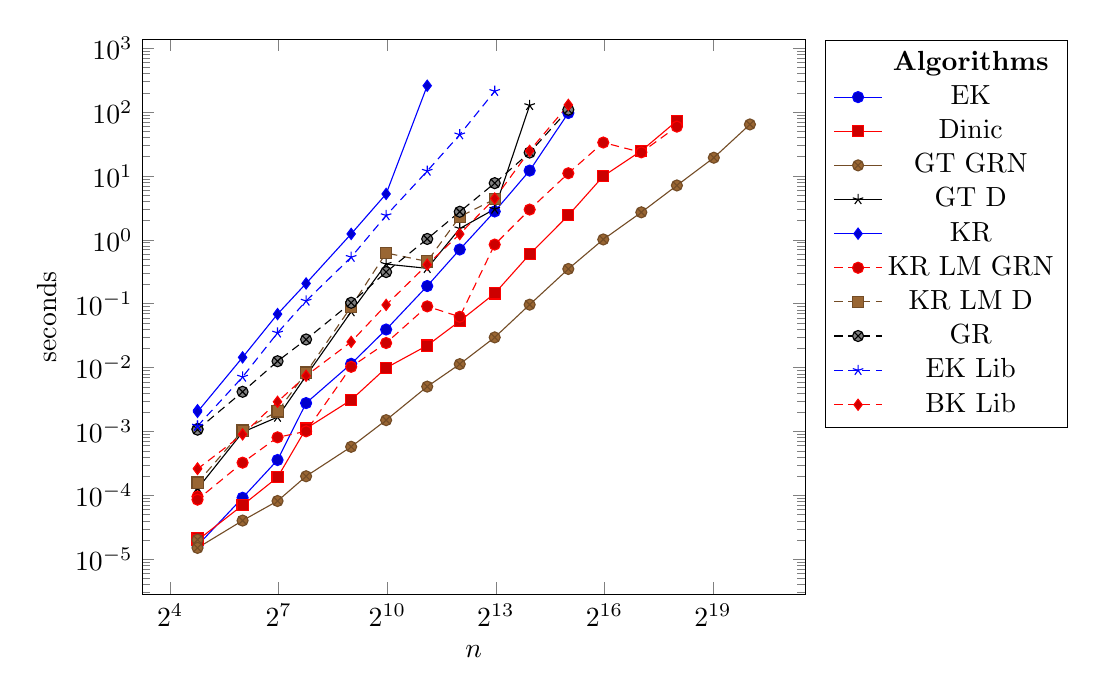
\begin{tikzpicture}
\begin{axis}[
    xlabel=$n$,ylabel=seconds,
    xmode=log,ymode=log,
    log basis x={2},
    legend style=
    {
        legend pos=outer north east
    },
    width=10cm
]
\addlegendimage{legend image code/.code=}
\legend{\textbf{Algorithms}, EK, Dinic, GT GRN, GT D, KR, KR LM GRN, KR LM D, GR, EK Lib, BK Lib}
\addplot table[x=n,y=value] {%EK
n value
27	1.83E-05
27	1.64353E-05
64	9.19488E-05
125	0.000358578
216	0.002789337
512	0.011478267
1000	0.039519567
2197	0.189271
4096	0.706506333
8000	2.78247
15625	12.12773333
32768	96.6569
};
\addplot table[x=n,y=value] {%Dinic
n value
27	2.16546E-05
27	1.98778E-05
64	7.04053E-05
125	0.000192226
216	0.001115157
512	0.003119373
1000	0.00991604
2197	0.0221898
4096	0.053542767
8000	0.144866667
15625	0.59337
32768	2.4171
64000	9.927513333
132651	24.71566667
262144	72.89203333
};
\addplot table[x=n,y=value] {%GT GRN
n value
27	2.03E-05
27	1.51027E-05
64	4.04221E-05
125	8.18436E-05
216	0.000199778
512	0.000577347
1000	0.001509167
2197	0.005050763
4096	0.0113486
8000	0.0297681
15625	0.096823533
32768	0.350279
64000	1.014996667
132651	2.6983
262144	7.101253333
531441	19.29156667
1061208	64.0214
};
\addplot table[x=n,y=value] {%GT D
n value
27	1.33E-04
27	0.000127152
64	0.000977459
125	0.00168207
216	0.007420783
512	0.0751745
1000	0.417246
2197	0.358329333
4096	1.503013333
8000	3.035766667
15625	127.1716667
};
\addplot table[x=n,y=value] {%KR
n value
27	2.16E-03
27	0.002033977
64	0.0144907
125	0.0688899
216	0.207899
512	1.23922
1000	5.23004
2197	258.178
};
\addplot table[x=n,y=value] {%KR LM GRN
n value
27	9.63E-05
27	8.59525E-05
64	0.000325931
125	0.000811551
216	0.001009107
512	0.010306333
1000	0.0242879
2197	0.090985567
4096	0.062492867
8000	0.84353
15625	2.978673333
32768	11.0194
64000	33.353
132651	23.40396667
262144	59.15526667
};
\addplot table[x=n,y=value] {%KR LM D
n value
27	1.61E-04
27	0.000158246
64	0.001037093
125	0.002061527
216	0.008381697
512	0.089949433
1000	0.622961333
2197	0.459367667
4096	2.298873333
8000	4.334706667
};
\addplot table[x=n,y=value] {%GR
n value
27	1.10E-03
27	0.00107007
64	0.004186893
125	0.0125998
216	0.027625867
512	0.103603333
1000	0.313361667
2197	1.03351
4096	2.753226667
8000	7.715346667
15625	23.232
32768	108.9246667
};
\addplot table[x=n,y=value] {%EK Lib
n value
27	0.001224103
27	0.001216997
64	0.007149513
125	0.0350155
216	0.110498333
512	0.535476
1000	2.40563
2197	11.93883333
4096	44.25053333
8000	211.9366667
};
\addplot table[x=n,y=value] {%BK Lib
n value
27	0.000264632
27	0.000259413
64	0.000902392
125	0.002922727
216	0.007462453
512	0.025325933
1000	0.095990433
2197	0.408633667
4096	1.230866667
8000	4.441643333
15625	24.72616667
32768	129.544
};
\end{axis}
\end{tikzpicture}
\caption{Best and worst results from the GenRmf square graphs}
\label{fig:GenRmf square_BW_Results}
\end{figure}

In the following sections we will discuss the performance of each algorithm, but the general performance can be seen from Figure~\ref{fig:GenRmf square_BW_Results}.

\subsection{Choosing $f(G)$ for the GRN Heuristic}
\label{GRNFGSection}

We implemented the GRN heuristic for the algorithms GT GRN, GT D GRN, KR LM GRN and KR LM D GRN. 
The reason we did not implement a KR D GRN algorithm is that previous tests have shown the KR D algorithm to have another bottleneck.
This bottleneck is discussed in Section~\ref{KingRaoResults}.

To find the best function, we tested each algorithm on graphs of the GenRmf and Wash types. 
On each size of graph in each family, we did an exponential search followed by a binary search for the best constant $f(G)=c$ for that particular graph and algorithm.
We did not test on CRE, CD or AK because no flow will have to be pushed back to source in those graphs, so the optimal solution would be to only do one global relabelling at the start of the algorithm.
We also did not test CRH because the construction of this graph is very special, and we believe that the GenRmf and Wash graphs are closer to a typical max flow problem.
Additionally, the GRC heuristic is already optimal for the CRH graphs, because it only does two global relabellings; one at the start, and one right after the minimum cut has been saturated.

We ran each test three times, which yielded about 180 tests per algorithm. We plotted these points, and used a regression tool to find the function on the form $f(G)=an^b$ that best describes the data.
This yielded the following equations

\begin{tabular}{|l|c|c|}
    \hline
    Algorithm & Function & $R^2$ \\\hline\hline
    GT GRN&$f(G)=1.8956n^{0.6548}$&$0.9442$\\\hline
    GT D GRN&$f(G)=0.54n^{0.7144}$&$0.9128$\\\hline
    KR LM GRN&$f(G)=1.5834n^{0.7578}$&$0.7824$\\\hline
    KR LM D GRN&$f(G)=1.6078n^{0.6509}$&$0.6219$\\\hline   
\end{tabular}
\\

Charts of the data points and the regression lines can be seen in Appendix~\ref{GRN_Functions}.




\subsection{Edmonds Karp}

The Edmonds Karp algorithm generally does not perform very well.
Dinic's algorithm is faster than Edmonds Karp, in all examples except for the AK graphs. 
This makes sense with respect to the worstcase time of $O(nm^2)$ for Edmonds Karp, and $O(n^2m)$ for Dinic.
We found that the running time of the Edmonds Karp algorithm is best described as a function of the number of augmenting paths, and the number of edges in the graph.
The more augmenting paths there are, the more breadth first searches will have to be done, and the time for each breath first search depends on the number of edges in the graph.
This is also why its worst case time is $O(nm^2)$. 


\begin{figure}[h]
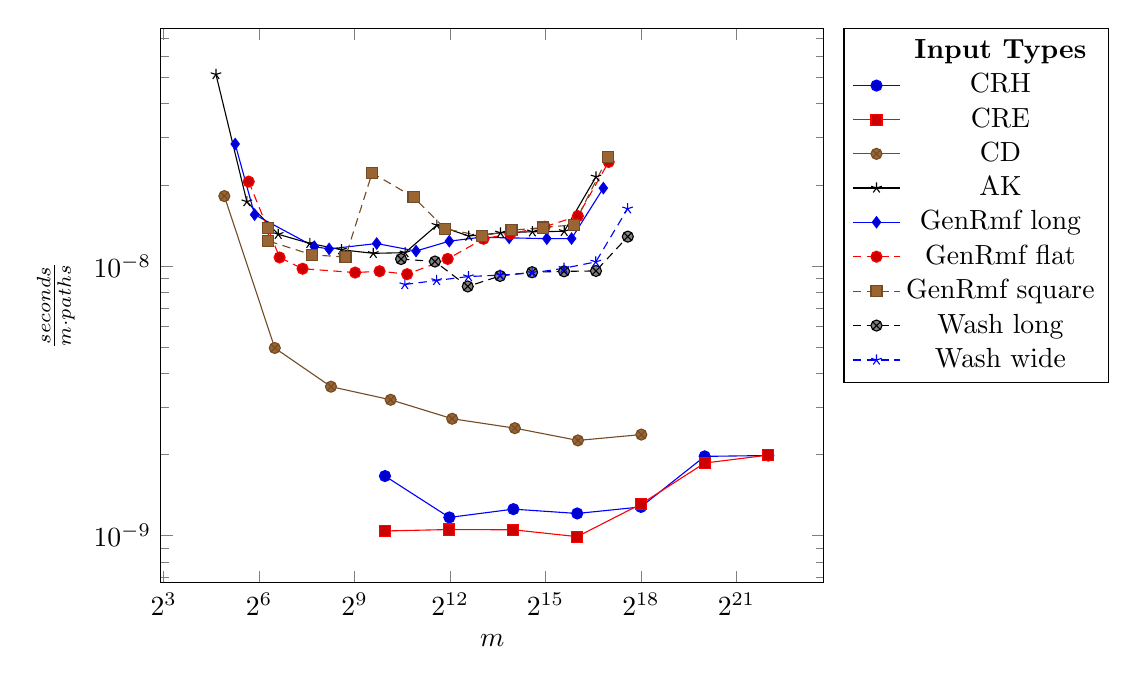
\begin{tikzpicture}
\begin{axis}[
    xlabel=$m$,ylabel=$\frac{\text{seconds}}{m\cdot \text{paths}}$,
    xmode=log,ymode=log,
    log basis x={2},
    legend style=
    {
        legend pos=outer north east
    },
    width=10cm
]
\addlegendimage{legend image code/.code=}
\legend{\textbf{Input Types}, CRH, CRE, CD, AK, GenRmf long, GenRmf flat, GenRmf square, Wash long, Wash wide}
\addplot table[x=n,y=value] {%CRH
n value
992	1.66466E-09
4032	1.16903E-09
16256	1.25451E-09
65280	1.2091E-09
261632	1.27864E-09
1047552	1.96903E-09
4192256	1.98336E-09
};
\addplot table[x=n,y=value] {%CRE
n value
992	1.0413E-09
4032	1.05426E-09
16256	1.05184E-09
65280	9.92107E-10
261632	1.31012E-09
1047552	1.85996E-09
4192256	1.99021E-09
};
\addplot table[x=n,y=value] {%CD
n value
30	1.81717E-08
90	4.96716E-09
306	3.57009E-09
1122	3.19207E-09
4290	2.71479E-09
16770	2.50517E-09
66306	2.25596E-09
263682	2.37129E-09
};
\addplot table[x=n,y=value] {%AK
n value
25	5.13295E-08
49	1.73307E-08
97	1.31136E-08
193	1.21362E-08
385	1.14906E-08
769	1.11464E-08
1537	1.12091E-08
3073	1.41778E-08
6145	1.29195E-08
12289	1.32742E-08
24577	1.34015E-08
49153	1.34511E-08
98305	2.14221E-08
};
\addplot table[x=n,y=value] {%GenRmf long
n value
38	2.83468E-08
58	1.55086E-08
213	1.17957E-08
294	1.15719E-08
828	1.21194E-08
1950	1.13672E-08
4026	1.23664E-08
7868	1.27728E-08
14840	1.27225E-08
33660	1.26353E-08
57717	1.26436E-08
115284	1.94512E-08
};
\addplot table[x=n,y=value] {%GenRmf flat
n value
51	2.05647E-08
100	1.07579E-08
165	9.77235E-09
518	9.45758E-09
882	9.56565E-09
1608	9.32887E-09
3888	1.0626E-08
8484	1.26209E-08
15232	1.31695E-08
32153	1.39854E-08
66150	1.53185E-08
129472	2.43192E-08
};
\addplot table[x=n,y=value] {%GenRmf square
n value
78	1.38184E-08
78	1.23946E-08
204	1.09934E-08
420	1.08071E-08
750	2.21376E-08
1848	1.80034E-08
3690	1.37307E-08
8268	1.29187E-08
15600	1.35717E-08
30780	1.38904E-08
60600	1.42187E-08
127968	2.5442E-08
};
\addplot table[x=n,y=value] {%Wash long
n value
1408	1.06141E-08
2944	1.03926E-08
6016	8.40057E-09
12160	9.18783E-09
24448	9.48726E-09
49024	9.55599E-09
98176	9.58903E-09
196480	1.28548E-08
};
\addplot table[x=n,y=value] {%Wash wide
n value
1528	8.54169E-09
3056	8.84407E-09
6112	9.14132E-09
12224	9.25413E-09
24448	9.42574E-09
48896	9.81213E-09
97792	1.03599E-08
195584	1.63099E-08
};
\end{axis}
\end{tikzpicture}
\caption{Edmonds and Karp performance per $m$ and the number of augmenting paths}
\label{fig:EK_runningTime}
\end{figure}

Figure~\ref{fig:EK_runningTime} shows the time for all measurements of Edmonds Karp, where the running time is divided by the product of the number of edges and the number of augmenting paths in the graph.
Since this chart is mostly flat, $m \cdot \text{\#AugmentingPaths}$ is a good approximation of the running time.
At $m=2^{16}$, the algorithm starts to exit L3 cache, which is the reason for the increase in running time for larger graphs.


\subsection{Dinic}

Dinic's algorithm generally performs well.
It generally beats the push relabel algorithms without heuristics, and many of the heuristics as well. It is not the fastest algorithm in any of our tests though.
It especially has problems on the AK and CD graphs. 
The AK graphs has a low number of augmenting paths in each layer graph. That means that doing a BFS to compute the layer graph, and then a DFS to find the flow in it is slower than just doing a few BFS's to find each augmenting path in the layer graph.
For this reason, we see EK perform better than Dinic on the AK graphs.

Our CRE and CRH graphs are easy for Dinic because there are never more than two layer graphs.
The CD graphs are designed to be hard for Dinic as it has $\Omega(n)$ layer graphs, and as many paths as we could fit in each layer graph. 
We made the CD graph, because we were missing a fully connected graph that Dinic struggles with. 
The results here are better than expected. Dinic does not perform as well as the GT algorithms, but it is not far behind.
The fact that Dinic was so efficient on CD graphs led us to conduct the previous analysis of the number of augmenting paths in the graph.
The observed number of augmenting paths found by Dinic fits well with the $m \log n$ bound achieved by the analysis.
When plotting $\mathrm{Paths}/m\log n$ all points lie on a horizontal line.



\begin{figure}[h]
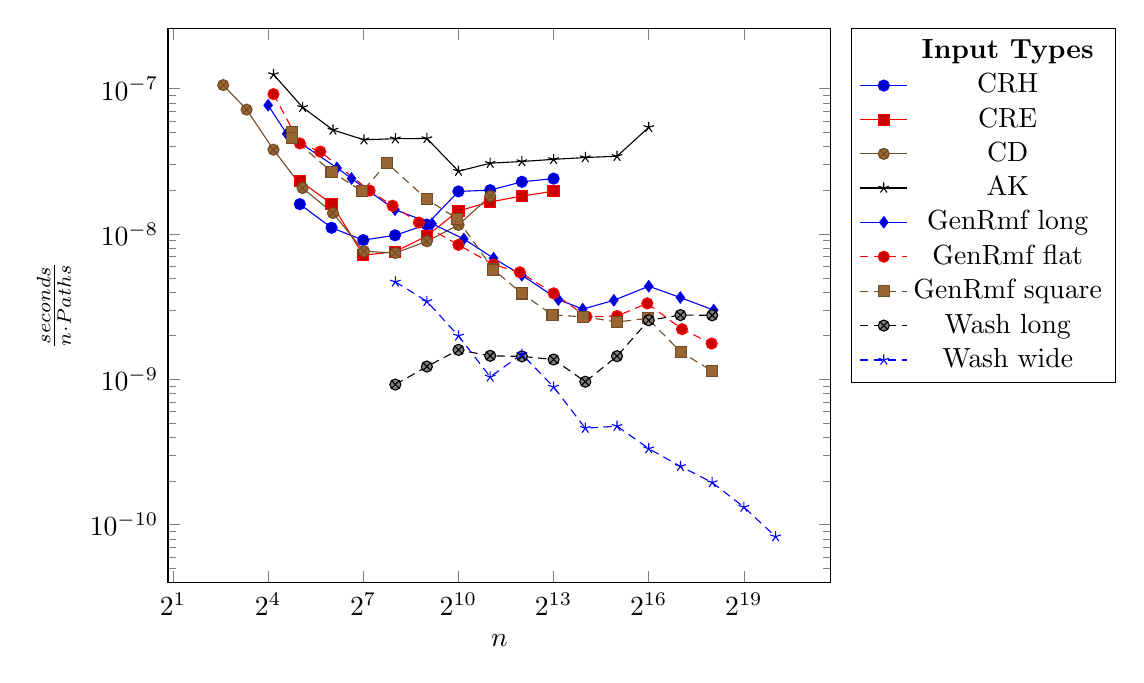
\begin{tikzpicture}
\begin{axis}[
    xlabel=$n$,ylabel=$\frac{\text{seconds}}{n\cdot \text{Paths}}$,
    xmode=log,ymode=log,
    log basis x={2},
    legend style=
    {
        legend pos=outer north east
    },
    width=10cm
]
\addlegendimage{legend image code/.code=}
\legend{\textbf{Input Types}, CRH, CRE, CD, AK, GenRmf long, GenRmf flat, GenRmf square, Wash long, Wash wide}
\addplot table[x=n,y=value] {%CRH
n value
32	1.60662E-08
64	1.10524E-08
128	9.09034E-09
256	9.8052E-09
512	1.16228E-08
1024	1.96589E-08
2048	2.00461E-08
4096	2.29003E-08
8192	2.40805E-08
};
\addplot table[x=n,y=value] {%CRE
n value
32	2.32243E-08
64	1.61998E-08
128	7.16023E-09
256	7.55879E-09
512	9.70943E-09
1024	1.44429E-08
2048	1.66357E-08
4096	1.82794E-08
8192	1.97247E-08
};
\addplot table[x=n,y=value] {%CD
n value
6	1.06002E-07
10	7.18898E-08
18	3.81028E-08
34	2.07454E-08
66	1.39579E-08
130	7.62282E-09
258	7.40559E-09
514	8.92618E-09
1026	1.1564E-08
2050	1.82553E-08
};
\addplot table[x=n,y=value] {%AK
n value
18	1.25445E-07
34	7.45452E-08
66	5.20575E-08
130	4.45512E-08
258	4.5328E-08
514	4.54889E-08
1026	2.71015E-08
2050	3.07429E-08
4098	3.15994E-08
8194	3.2674E-08
16386	3.36491E-08
32770	3.43191E-08
65538	5.42947E-08
};
\addplot table[x=n,y=value] {%GenRmf long
n value
16	7.70404E-08
24	4.90468E-08
72	2.85335E-08
99	2.41266E-08
256	1.47136E-08
575	1.17925E-08
1152	9.25426E-09
2205	6.82108E-09
4096	5.21221E-09
9100	3.54137E-09
15488	3.04506E-09
30589	3.50078E-09
65536	4.37844E-09
130682	3.65803E-09
270848	2.99932E-09
};
\addplot table[x=n,y=value] {%GenRmf flat
n value
18	9.18556E-08
32	4.20773E-08
50	3.69572E-08
147	1.99257E-08
243	1.5665E-08
432	1.19976E-08
1024	8.43176E-09
2205	6.16549E-09
3920	5.46192E-09
8214	3.90928E-09
16807	2.70144E-09
32768	2.72785E-09
63504	3.33529E-09
135531	2.21539E-09
259308	1.76556E-09
};
\addplot table[x=n,y=value] {%GenRmf square
n value
27	5.01265E-08
27	4.60135E-08
64	2.68313E-08
125	1.97155E-08
216	3.07307E-08
512	1.74072E-08
1000	1.27292E-08
2197	5.6998E-09
4096	3.90324E-09
8000	2.77607E-09
15625	2.69714E-09
32768	2.48514E-09
64000	2.62866E-09
132651	1.5397E-09
262144	1.14193E-09
};
\addplot table[x=n,y=value] {%Wash long
n value
258	9.21744E-10
514	1.22555E-09
1026	1.59596E-09
2050	1.45298E-09
4098	1.44002E-09
8194	1.37073E-09
16386	9.63818E-10
32770	1.4445E-09
65538	2.55088E-09
131074	2.77054E-09
262146	2.75927E-09
};
\addplot table[x=n,y=value] {%Wash wide
n value
258	4.6875E-09
514	3.44298E-09
1026	1.9923E-09
2050	1.03997E-09
4098	1.49151E-09
8194	8.8731E-10
16386	4.61535E-10
32770	4.76501E-10
65538	3.33716E-10
131074	2.52127E-10
262146	1.95298E-10
524290	1.32129E-10
1048578	8.27744E-11
};
\end{axis}
\end{tikzpicture}
\caption{Dinic performance per $nP$}
\label{fig:Dinic_runningTime}
\end{figure}

With regard to the running time, we found that the running time of Dinic was mostly proportional to $n$ times the total number of paths the algorithm found.
This can be seen on Figure~\ref{fig:Dinic_runningTime}.
Here we divided the running time in each test by $n\cdot \text{Paths}$.
Many of the graphs, such as the GenRmf and Wash graphs, seems to be faster than $n\cdot\text{Paths}$. 
We believe the problem is that not all paths are of length $n$. For many of the layer graphs, $k$ is a lot smaller than $n$.
In fact, as $k$ approach $n$, the layer graph will not be able to contain as many paths as when $k$ is significantly smaller than $n$.
For example, if $k=n$, there can only be one augmenting path that contains all nodes.
This means that $n$ is an over estimation on the average length of the augmenting paths.

\subsection{Goldberg Tarjan}

The Goldberg Tarjan algorithms perform very well, especially with the heuristics.
Before the heuristics, GT was the fastest on the CRE, CD and AK graphs. 
With heuristics, in all our tests, it is always some version of GT that is the fastest.

It makes good sense that GT is the fastest on the CRE, CD and AK graphs. CRE is basically the best case graph for GT, because it can ignore the majority of all the edges due to the fact that nodes never go above a label of 2.
The reason the maximum label is two is that a node is only relabelled from $1$ to $2$ when no more flow can be sent to the target node.
The graph is fully connected with very high capacities, so once a node has been relabelled to $2$, it will be able to send all its excess to a node with label $1$.

The GRH graphs on the other hand is the worst case for this algorithm.
All nodes will have to be relabelled to $n$ before the algorithm can terminate. In-between the relabels, the algorithm will also spend time pushing the excess back and forth between nodes.
That is why, without heuristics, the GT algorithm falls far behind Dinic on the CRH graphs.

The Goldberg Tarjan algorithm has an advantage in the CD graphs, because no flow will ever have to be pushed back to source. 
The way the CD graphs are constructed, no edge has more capacity than what is needed to get the flow to the target node.
The maximum label depends on the order the algorithm processes the nodes. For each CD graph, there is one order which results in no nodes getting a label higher than $2$.
There is also an order that results in nodes having labels $n$, $n-1$, $n-2$, etc. Regardless of the label, the same number of pushes is required though.



\begin{figure}[h]
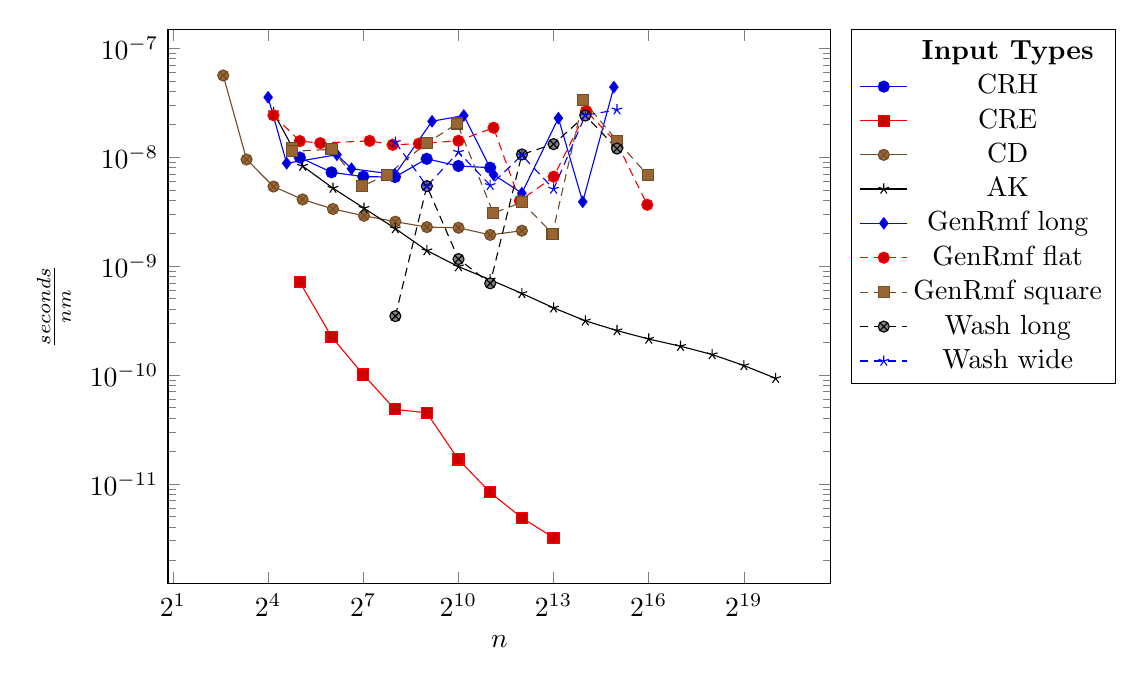
\begin{tikzpicture}
\begin{axis}[
    xlabel=$n$,ylabel=$\frac{\text{seconds}}{nm}$,
    xmode=log,ymode=log,
    log basis x={2},
    legend style=
    {
        legend pos=outer north east
    },
    width=10cm
]
\addlegendimage{legend image code/.code=}
\legend{\textbf{Input Types}, CRH, CRE, CD, AK, GenRmf long, GenRmf flat, GenRmf square, Wash long, Wash wide}
\addplot table[x=n,y=value] {%CRH
n value
32	9.90712E-09
64	7.24742E-09
128	6.61376E-09
256	6.56429E-09
512	9.63395E-09
1024	8.2859E-09
2048	7.99078E-09
};
\addplot table[x=n,y=value] {%CRE
n value
32	7.1015E-10
64	2.24209E-10
128	1.00655E-10
256	4.82229E-11
512	4.48739E-11
1024	1.67318E-11
2048	8.34562E-12
4096	4.86383E-12
8192	3.20329E-12
};
\addplot table[x=n,y=value] {%CD
n value
6	5.61416E-08
10	9.50089E-09
18	5.36295E-09
34	4.08415E-09
66	3.33572E-09
130	2.89291E-09
258	2.55076E-09
514	2.27462E-09
1026	2.24389E-09
2050	1.92973E-09
4098	2.10844E-09
};
\addplot table[x=n,y=value] {%AK
n value
18	2.56647E-08
34	8.26537E-09
66	5.18647E-09
130	3.39477E-09
258	2.20466E-09
514	1.38395E-09
1026	9.86652E-10
2050	7.47385E-10
4098	5.60005E-10
8194	4.12565E-10
16386	3.13874E-10
32770	2.54984E-10
65538	2.13448E-10
131074	1.83323E-10
262146	1.53786E-10
524290	1.21857E-10
1048578	9.30332E-11
};
\addplot table[x=n,y=value] {%GenRmf long
n value
16	3.54335E-08
24	8.77545E-09
72	1.05068E-08
99	7.81762E-09
256	6.92696E-09
575	2.13165E-08
1152	2.40867E-08
2205	6.90549E-09
4096	4.66368E-09
9100	2.27639E-08
15488	3.88656E-09
30589	4.39229E-08
};
\addplot table[x=n,y=value] {%GenRmf flat
n value
18	2.41938E-08
32	1.402E-08
50	1.34336E-08
147	1.40864E-08
243	1.29601E-08
432	1.32838E-08
1024	1.41106E-08
2205	1.8587E-08
3920	3.968E-09
8214	6.60992E-09
16807	2.63829E-08
32768	1.34006E-08
63504	3.647E-09
};
\addplot table[x=n,y=value] {%GenRmf square
n value
27	1.20752E-08
27	1.12842E-08
64	1.17888E-08
125	5.41498E-09
216	6.87753E-09
512	1.34166E-08
1000	2.0345E-08
2197	3.04784E-09
4096	3.8493E-09
8000	1.98347E-09
15625	3.31797E-08
32768	1.41112E-08
64000	6.83458E-09
};
\addplot table[x=n,y=value] {%Wash long
n value
258	3.46356E-10
514	5.40945E-09
1026	1.15649E-09
2050	6.92953E-10
4098	1.05799E-08
8194	1.31438E-08
16386	2.40597E-08
32770	1.19685E-08
};
\addplot table[x=n,y=value] {%Wash wide
n value
258	1.36924E-08
514	5.40668E-09
1026	1.11032E-08
2050	5.50623E-09
4098	1.03918E-08
8194	5.09109E-09
16386	2.41668E-08
32770	2.72197E-08
};
\end{axis}
\end{tikzpicture}
\caption{GT performance per $nm$}
\label{fig:GT_runningTime}
\end{figure}

\begin{figure}[h]
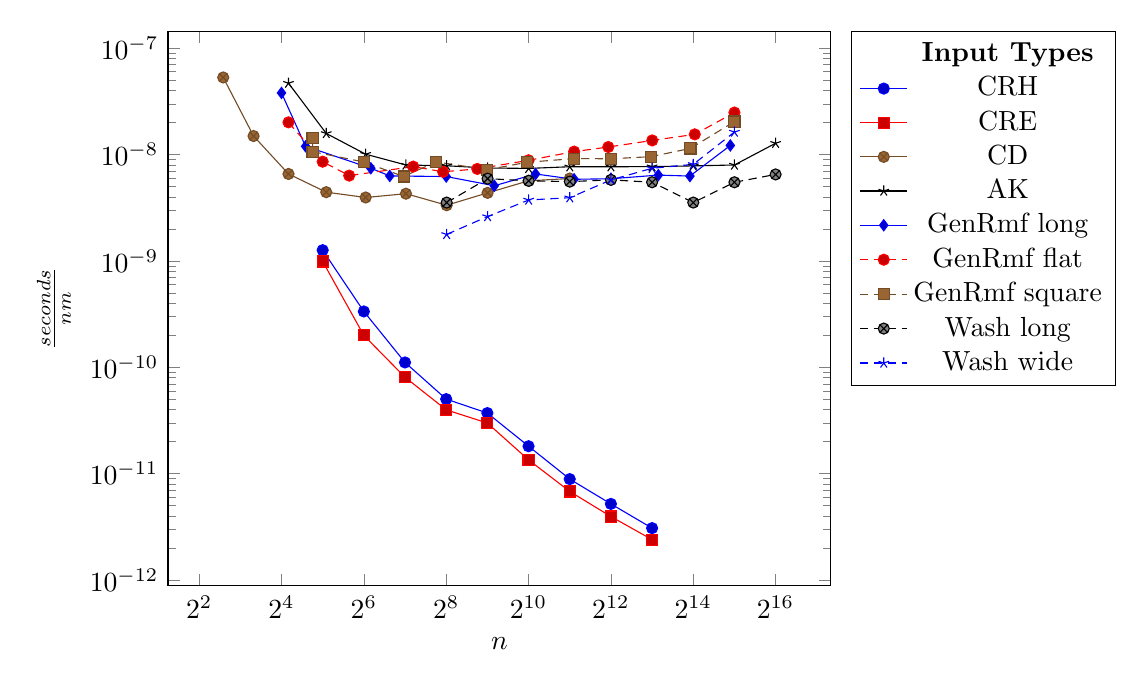
\begin{tikzpicture}
\begin{axis}[
    xlabel=$n$,ylabel=$\frac{\text{seconds}}{nm}$,
    xmode=log,ymode=log,
    log basis x={2},
    legend style=
    {
        legend pos=outer north east
    },
    width=10cm
]
\addlegendimage{legend image code/.code=}
\legend{\textbf{Input Types}, CRH, CRE, CD, AK, GenRmf long, GenRmf flat, GenRmf square, Wash long, Wash wide}
\addplot table[x=n,y=value] {%CRH
n value
32	1.26288E-09
64	3.35238E-10
128	1.11168E-10
256	5.03027E-11
512	3.71824E-11
1024	1.81421E-11
2048	8.90429E-12
4096	5.20555E-12
8192	3.0819E-12
};
\addplot table[x=n,y=value] {%CRE
n value
32	9.90013E-10
64	1.9968E-10
128	8.07477E-11
256	3.98834E-11
512	2.99502E-11
1024	1.35027E-11
2048	6.81994E-12
4096	3.96241E-12
8192	2.40243E-12
};
\addplot table[x=n,y=value] {%CD
n value
6	5.30569E-08
10	1.49299E-08
18	6.57264E-09
34	4.43056E-09
66	3.94952E-09
130	4.2887E-09
258	3.3403E-09
514	4.36561E-09
1026	5.66833E-09
2050	5.95279E-09
};
\addplot table[x=n,y=value] {%AK
n value
18	4.68876E-08
34	1.57975E-08
66	1.0078E-08
130	7.98015E-09
258	7.84601E-09
514	7.4766E-09
1026	7.41183E-09
2050	7.68286E-09
4098	7.68821E-09
8194	7.69572E-09
16386	7.82987E-09
32770	7.98256E-09
65538	1.27783E-08
};
\addplot table[x=n,y=value] {%GenRmf long
n value
16	3.79906E-08
24	1.19665E-08
72	7.4366E-09
99	6.29532E-09
256	6.21655E-09
575	5.09247E-09
1152	6.56912E-09
2205	5.85557E-09
4096	5.92566E-09
9100	6.41111E-09
15488	6.27912E-09
30589	1.21796E-08
};
\addplot table[x=n,y=value] {%GenRmf flat
n value
18	2.00808E-08
32	8.57161E-09
50	6.33991E-09
147	7.7075E-09
243	6.89168E-09
432	7.32937E-09
1024	8.83296E-09
2205	1.06628E-08
3920	1.1773E-08
8214	1.3578E-08
16807	1.54848E-08
32768	2.48237E-08
};
\addplot table[x=n,y=value] {%GenRmf square
n value
27	1.43953E-08
27	1.06515E-08
64	8.51412E-09
125	6.22088E-09
216	8.53572E-09
512	7.21217E-09
1000	8.45903E-09
2197	9.16498E-09
4096	9.1337E-09
8000	9.54867E-09
15625	1.14186E-08
32768	2.04167E-08
};
\addplot table[x=n,y=value] {%Wash long
n value
258	3.53846E-09
514	5.93937E-09
1026	5.66374E-09
2050	5.56832E-09
4098	5.78294E-09
8194	5.49482E-09
16386	3.53918E-09
32770	5.49036E-09
65538	6.50731E-09
};
\addplot table[x=n,y=value] {%Wash wide
n value
258	1.77663E-09
514	2.61444E-09
1026	3.74229E-09
2050	3.93122E-09
4098	5.77718E-09
8194	7.43357E-09
16386	8.0869E-09
32770	1.62903E-08
};
\end{axis}
\end{tikzpicture}
\caption{GT GRC performance per $nm$}
\label{fig:GT_GRC_runningTime}
\end{figure}

The algorithm will have to push flow back to the source in the AK graph, but this is only for the two nodes right next to the source.
All other nodes is able to push all their excess to the target node, so the algorithm won't have to spend time relabelling a lot of nodes to get flow back to the source.
There are long paths in the graph though, so labels get high even though all the excess is pushed to the target.


It seems apparent that the running time of the GT algorithm is directly proportional to the number of relabels required.
When we try to compare it to $O(n^3)$ or $O(nm)$, we get a lot of big jumps up and down in the results.
This tells us that there is something other than $n$ and $m$ that has a big impact on the running time.
As can be seen from Figure~\ref{fig:GT_runningTime}, the jumps comes from the GenRmf and Washington graphs. 
We found that the jumps are caused by the randomized capacities in the GenRmf and Washington.
If we consider the minimum cut in such a graph, which is an $(S, T)$ cut, then the problem is that the size of the set $S$ can get very big.
All nodes in $S$ would have to be relabelled above $n$ in order for the excess to be sent back to $s$.
This means that if the size of $S$ is big in one graph and small in another, even though the second graph is bigger than the first, 
the second graph could be solved faster.


This is the reason we decided to implement the global relabelling heuristics. 
As can be seen from Figure~\ref{fig:GT_GRC_runningTime}, the jumps disappeared when we implemented the GRC heuristic.
This is because the algorithm no longer has to relabel the nodes in $S$ all the way to $n$ one step at the time.

Based on the data in Figure~\ref{fig:GT_runningTime}, it seems that the GT algorithm is a faster than $nm$ for the AK and CRE graphs.
CD and CRH graphs seems to be levelling out towards the end of their chart, but we do not have enough points to be sure. 
It would seem that $nm$ is a better estimate for the running time of GT than the worst case bound of $O(n^3)$ in our test data.

The GT D algorithm has the same jumps as the GT algorithm. 
The effect of dynamic trees are described in Section~\ref{Dynamic Trees Section}.
Additionally, the benefits and drawbacks of the different heuristics are described in Section~\ref{Global Relabelling Section}.

\subsection{King Rao}
\label{KingRaoResults}

The KR D, KR D GRC, KR D GRP algorithms are the worst algorithms in every test we have done.
The problem is that the game requires $2n^2$ nodes and $nm$ edges.
This results in the issue that every time a node is relabelled, a new node in the game will have to be loaded from main memory, or possibly even the hard disk.
We do however not have any examples where the algorithm went to the disk, because it failed with a memory allocation error for large inputs.
The performance is only worse when going to the disk, so running for larger inputs will not yield any new information. For this reason, we did not want to investigate this error further.
We did not see any major improvements when using the GRC or GRP heuristics on this algorithm.
As mentioned in Section~\ref{HeuristicsSection}, the problem is that we can not efficiently relabel a node multiple steps at a time since the data structure has to be updated for all the labels in-between.
These three algorithms perform about the same in all of our tests. An example can be seen in Figure~\ref{fig:GenRmf long_KR_Results}.
Since there is no benefit from the other heuristics, we decided not to spend time on implementing the GRN heuristic for the KR D algorithm.



\begin{figure}[h]
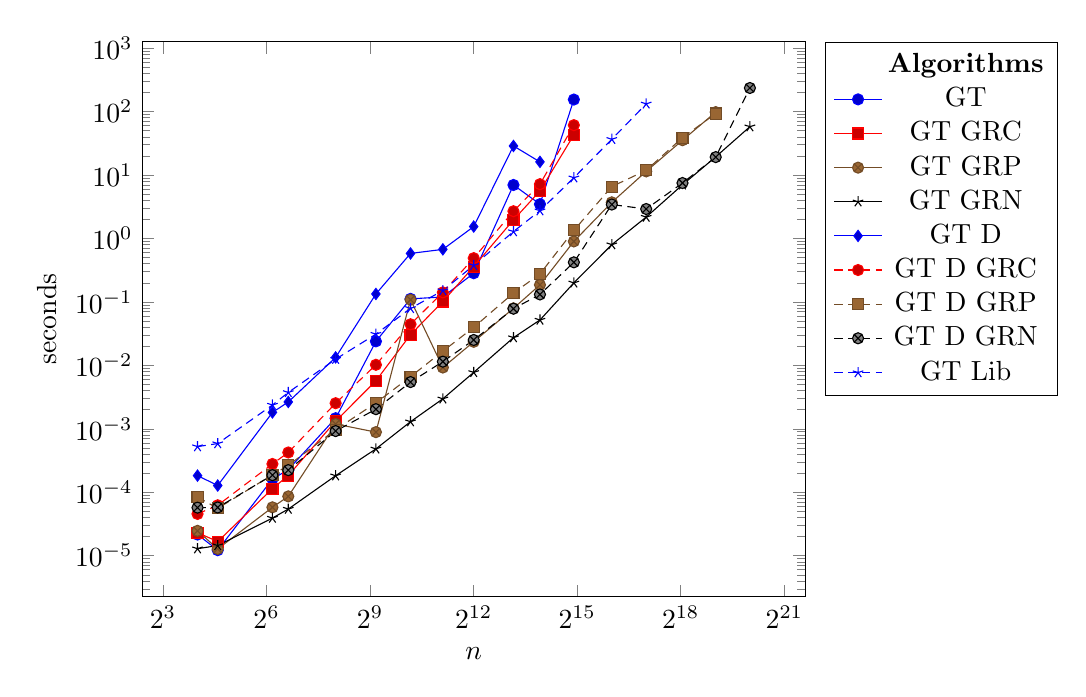
\begin{tikzpicture}
\begin{axis}[
    xlabel=$n$,ylabel=seconds,
    xmode=log,ymode=log,
    log basis x={2},
    legend style=
    {
        legend pos=outer north east
    },
    width=10cm
]
\addlegendimage{legend image code/.code=}
\legend{\textbf{Algorithms}, GT, GT GRC, GT GRP, GT GRN, GT D, GT D GRC, GT D GRP, GT D GRN, GT Lib}
\addplot table[x=n,y=value] {%GT
n value
16	2.15436E-05
24	1.22154E-05
72	0.000161133
99	0.00022754
256	0.001468293
575	0.023901133
1152	0.111713
2205	0.119803
4096	0.28348
9100	6.972716667
15488	3.47428
30589	154.8906667
};
\addplot table[x=n,y=value] {%GT GRC
n value
16	2.30983E-05
24	1.66574E-05
72	0.000114048
99	0.000183232
256	0.00131771
575	0.005709937
1152	0.030467267
2205	0.101588
4096	0.360189
9100	1.96376
15488	5.613036667
30589	42.95033333
};
\addplot table[x=n,y=value] {%GT GRP
n value
16	2.4653E-05
24	1.27707E-05
72	5.78567E-05
99	8.60632E-05
256	0.001188007
575	0.000886396
1152	0.108298
2205	0.009246077
4096	0.0235188
9100	0.079296967
15488	0.185714333
30589	0.899061333
65536	3.712403333
130682	11.41563333
270848	35.41273333
527796	98.1075
};
\addplot table[x=n,y=value] {%GT GRN
n value
16	1.28818E-05
24	1.44365E-05
72	3.92005E-05
99	5.43033E-05
256	0.000182232
575	0.000482289
1152	0.001294393
2205	0.002970023
4096	0.00775149
9100	0.0273884
15488	0.051847533
30589	0.199656667
65536	0.799864667
130682	2.173773333
270848	7.017736667
527796	19.36696667
1048576	57.80963333
};
\addplot table[x=n,y=value] {%GT D
n value
16	0.000182899
24	0.000127707
72	0.001811667
99	0.002649647
256	0.01333294
575	0.133493
1152	0.581190667
2205	0.673778667
4096	1.540246667
9100	28.75023333
15488	16.11123333
};
\addplot table[x=n,y=value] {%GT D GRC
n value
16	4.55303E-05
24	6.22988E-05
72	0.000279179
99	0.000423655
256	0.00253193
575	0.010205033
1152	0.044468633
2205	0.141443667
4096	0.490048
9100	2.690203333
15488	7.183683333
30589	61.1455
};
\addplot table[x=n,y=value] {%GT D GRP
n value
16	8.40646E-05
24	5.57469E-05
72	0.000188007
99	0.000264631
256	0.000967909
575	0.002560693
1152	0.006632443
2205	0.016727867
4096	0.039698667
9100	0.138222667
15488	0.27566
30589	1.342566667
65536	6.573553333
130682	11.86123333
270848	38.87526667
527796	93.12866667
};
\addplot table[x=n,y=value] {%GT D GRN
n value
16	5.71906E-05
24	5.75237E-05
72	0.000186008
99	0.000223099
256	0.000920491
575	0.002039097
1152	0.005452093
2205	0.011442267
4096	0.025133533
9100	0.078167533
15488	0.131162333
30589	0.420732667
65536	3.42981
130682	2.91399
270848	7.486506667
527796	19.16753333
1048576	235.5196667
};
\addplot table[x=n,y=value] {%GT Lib
n value
16	0.000524045
24	0.000584789
72	0.002370587
99	0.003742273
256	0.012512867
575	0.031066333
1152	0.079139833
2205	0.151054
4096	0.376943
9100	1.286306667
15488	2.73918
30589	9.066496667
65536	36.64306667
130682	132.3713333
};
\end{axis}
\end{tikzpicture}
\caption{Goldberg and Tarjan results from the GenRmf long graphs}
\label{fig:GenRmf long_GT_Results}
\end{figure}


\begin{figure}[h]
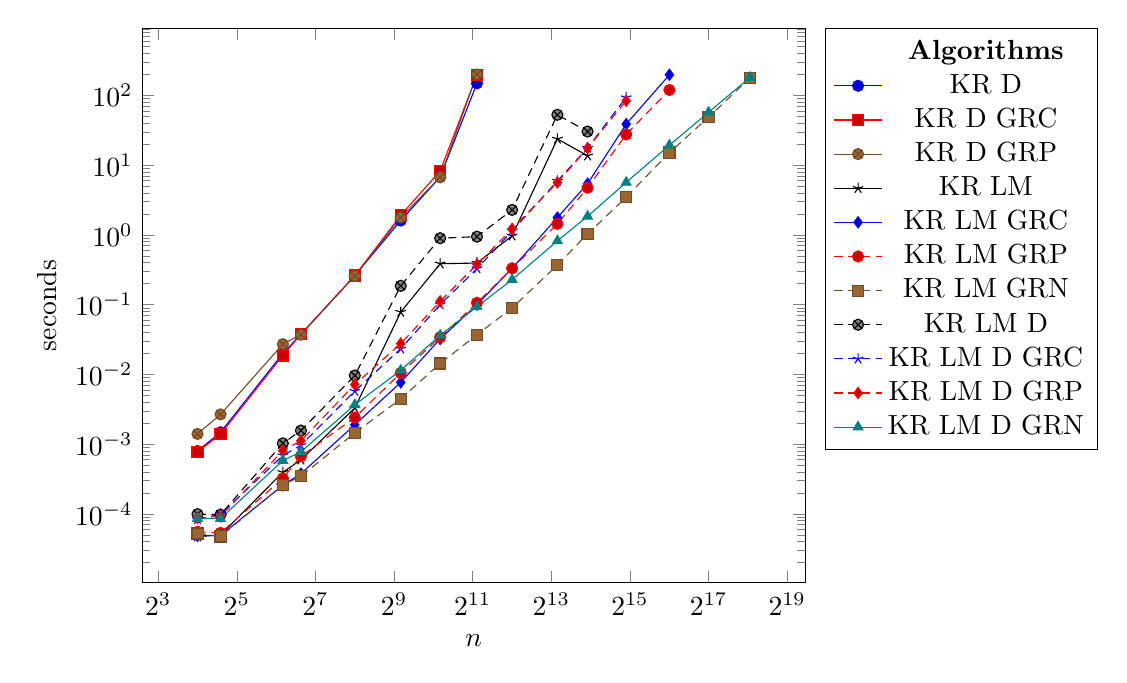
\begin{tikzpicture}
\begin{axis}[
    xlabel=$n$,ylabel=seconds,
    xmode=log,ymode=log,
    log basis x={2},
    legend style=
    {
        legend pos=outer north east
    },
    width=10cm
]
\addlegendimage{legend image code/.code=}
\legend{\textbf{Algorithms}, KR D, KR D GRC, KR D GRP, KR LM, KR LM GRC, KR LM GRP, KR LM GRN, KR LM D, KR LM D GRC, KR LM D GRP, KR LM D GRN}
\addplot table[x=n,y=value] {%KR
n value
16	0.000795004
24	0.00147618
72	0.019901867
99	0.037501367
256	0.260456667
575	1.606663333
1152	6.740186667
2205	149.337
};
\addplot table[x=n,y=value] {%KR GRC
n value
16	0.000769905
24	0.001389337
72	0.018663067
99	0.0377529
256	0.261381
575	1.908376667
1152	8.252073333
2205	197.4756667
};
\addplot table[x=n,y=value] {%KR GRP
n value
16	0.00139845
24	0.002666637
72	0.0271098
99	0.037121367
256	0.258182333
575	1.773686667
1152	6.72207
2205	200.141
};
\addplot table[x=n,y=value] {%KR LM
n value
16	4.70851E-05
24	4.97503E-05
72	0.000394004
99	0.000594782
256	0.003290843
575	0.078265033
1152	0.385737667
2205	0.395114667
4096	0.969813
9100	23.78033333
15488	13.6657
};
\addplot table[x=n,y=value] {%KR LM GRC
n value
16	4.81955E-05
24	4.90839E-05
72	0.000255858
99	0.000376681
256	0.001889957
575	0.007676197
1152	0.0321853
2205	0.099800333
4096	0.331238
9100	1.773373333
15488	5.421613333
30589	38.8194
65536	197.752
};
\addplot table[x=n,y=value] {%KR LM GRP
n value
16	5.53027E-05
24	5.31928E-05
72	0.000322266
99	0.000671628
256	0.002406003
575	0.010445347
1152	0.034050267
2205	0.10638
4096	0.331282667
9100	1.439603333
15488	4.751253333
30589	27.6015
65536	119.7773333
};
\addplot table[x=n,y=value] {%KR LM GRN
n value
16	5.21933E-05
24	4.73072E-05
72	0.000259523
99	0.000345365
256	0.001449643
575	0.00443921
1152	0.014312
2205	0.037018833
4096	0.089594333
9100	0.369817
15488	1.033306667
30589	3.473556667
65536	15.1593
130682	48.64013333
270848	178.9876667
};
\addplot table[x=n,y=value] {%KR LM D
n value
16	9.88343E-05
24	9.73907E-05
72	0.001024097
99	0.001562027
256	0.009612567
575	0.186065333
1152	0.896549
2205	0.943830667
4096	2.28156
9100	52.7981
15488	30.36093333
};
\addplot table[x=n,y=value] {%KR LM D GRC
n value
16	8.31763E-05
24	9.87233E-05
72	0.000685843
99	0.000960468
256	0.00575304
575	0.023246133
1152	0.100415667
2205	0.328566333
4096	1.139136667
9100	5.931156667
15488	17.6933
30589	93.37536667
};
\addplot table[x=n,y=value] {%KR LM D GRP
n value
16	8.69519E-05
24	9.19491E-05
72	0.000803777
99	0.001117273
256	0.007166817
575	0.027587633
1152	0.111327333
2205	0.376117333
4096	1.221456667
9100	5.651543333
15488	17.5763
30589	83.79273333
};
\addplot[mark=triangle*, teal] table[x=n,y=value] {%KR LM D GRN
n value
16	8.53971E-05
24	8.53972E-05
72	0.000580235
99	0.000774794
256	0.00366275
575	0.011421333
1152	0.036280633
2205	0.0934643
4096	0.228176333
9100	0.820808667
15488	1.847203333
30589	5.658126667
65536	19.2994
130682	57.2744
270848	180.989
};
\end{axis}
\end{tikzpicture}
\caption{King and Rao results from the GenRmf long graphs}
\label{fig:GenRmf long_KR_Results}
\end{figure}


The LM versions behave similar to the corresponding GT algorithms, except that they are slower.
A good example of this can be seen from comparing Figure~\ref{fig:GenRmf long_GT_Results} with Figure~\ref{fig:GenRmf long_KR_Results}. 
If you look at KR LM and KR LM D in Figure~\ref{fig:GenRmf long_KR_Results} and compare the curves to GT and GT D in Figure~\ref{fig:GenRmf long_GT_Results}, you see that the curves have the same ups and downs, but the KR algorihms are slower.
The main difference between the GT algorithms and the KR LM algorithms is the choice of current edges.
In our tests, the overhead that results from the more complicated way of choosing current edges is far greater than any time saved.
We have no example where the fastest KR algorithm beats the fastest GT algorithm, but KR LM D does beat GT D on GenRmf and Wash graphs.

When we first ran our different implementations of the King Rao algorithm, we observed big differences in running time between runs on the same graph, especially on the AK graphs.
As an example, when we tested KR LM D GRP on an AK graph with $n=8194$, we got results in the range from $0.21$ seconds to $6.61$ seconds.
This was unexpected, since the algorithm is not randomized, and it is the exact same input. 
We managed to track the issue down to the initial sorting of the edges according to unsigned capacity. 
We used the implementation of quick sort from the c++ library, which is not a stable sort. If two edges have the same unsigned capacity, the position of them relative to each other is random.
We managed to get consistent results by making sure that the comparator we use never returns $0$. With this, we got the example above down to $0,06$ seconds.
This shows that the order in which the edges are added has a very big impact on the running time. 
It affects in the order in which nodes a processed, because the act of adding an edge modifies the amount of visible edges on the nodes next to the edge.
In the AK graphs, many edges have the same capacity, so the the issue can have a very big effect on graphs of this type.
The results displayed for the KR algorithms in the charts are results from after we made the sorting deterministic.

\subsection{Goldberg Rao}

The GR algorithm is slower than most of our other algorithms.
The only algorithms that are consistently worse than GR are the KR algorithms without memory optimizations.
On some graphs, GR does beat the KR LM and GT algorithms without heuristics on large inputs.
We think that the reasons that GR is so slow compared to the other algorithm is mainly that it is doing a lot of different things, 
which means it has allocated a lot more memory than the others. 
All the memory is being used at some point in the main loop of the algorithm, so it will have to swap memory between caches more often than the other algorithms.
Also, we have not spent much time on locating and removing bottlenecks in this algorithm or on tweaking the constants.

Tweaking the constants is something we think could make a big difference.
We see big differences in the running time of GR on long and wide GenRmf graphs.
On GenRmf graphs, the edges within each layer has capacities $10000a^2$, which is needed to route all flow that could be sent between layers.
The first cut of the graph used to bound $F$ in the algorithm is going to be made between $s$ and the rest of the graph.
This cut contains two edges with $10000a^2$ capacity and one edge with a random capacity up to 10000.
So after the first iteration, $F=20000a^2$, which influences $\Delta$.
On long GenRmf graphs, $b=a^2$, which means that $a$ is and by extension the capacities on the edges inside the layers are small compared to capacities on edges between layers.
This causes $F$ and by extension $\Delta$ to be very small after the first iteration. 
The differences in capacity on edges inside layers and edges between layers is so small that after saturating an edge between each layer, all nodes become a single connected component.
That means that in the majority of the iterations, the algorithm does not run the blocking flow algorithm, but just routes $\Delta$ flow inside the big connected component.

On the wide GenRmf graphs however, edges inside the layers have a very big capacity compared to the edges between the layers.
This causes $F$ and by extension $\Delta$ to be so big that only edges inside layers are going to be zero length arcs.
The first layer graph where connected components are formed will be single list of super nodes.

In both cases, we can send about $5000a^2$ on average between the cuts. 
We are only allowed to send $\Delta = F/\Lambda = 20000a^2/\Lambda$ units of flow from $s$ to $t$.
Since GenRmf graphs are very sparse, we get $\Lambda=\sqrt{m}=O(\sqrt{n})$.
So when $n>16$, $\Delta$ becomes so small that we are not allowed to send $5000a^2$ units of flow, which means we wont be able to send the max flow in the first iterations.

If we experimented with other values of $\Delta$, we could get the wide GenRmf graphs to solve the max flow problem in very few steps.
In the wide GenRmf graphs, the layer graph will consist of a single path of super nodes, and the minimum cut will be between two of them.
If $\Delta$ allowed this cut to be saturated, the algorithm would be finished.
 
We see a similar story in the wash graphs. In the long version, the cuts contain few edges which results in a low $\Delta$ compared to the capacity on the edges 
as opposed to the wide version where there is a lot of edges in the cuts.
Also here, the long version with the relatively low $\Delta$ is faster.
After flow has been sent on a path $(s, v_1, \ldots, v_k, t)$ in the long version, a connected component can form from the smallest 
$i$ and largest $j$ such that there is an alternate path from $v_i$ to $v_j$.
Any other alternate paths from $v_k$ to $v_l$ where $i\leq k < l \leq j$ would also be part of that connected component.
As soon as two connected components share a node, they become one connected component.
This results in very quickly getting the entire graph into one connected component.

What takes time depends heavily on how $\Delta$ is in relation to the capacities on the edges, which affects how strongly connected components are formed.
In graphs that almost only consist of strongly connected components, we naturally see almost no time spent on the blocking flow algorithm.
Vice versa, if the graph has few strongly connected components, a lot of the time is spent on the blocking flow algorithm.
If we compare GenRmf long, wide and square graphs of the same size, then GR is fastest on the long graphs and slowest on the wide graphs with the square ones in between.
We would like to have some input graphs where we can vary the number and size of connected components without changing the result of the algorithm or the resulting flow graph.
That would give us a more clear image of the trade off between spending time on connected components and spending time on the blocking flow algorithm.
Based on the results we have now, it would seem that bigger is better in terms of strongly connected components.


\subsection{Dynamic Trees}
\label{Dynamic Trees Section}
Dynamic trees tend to make the running time op the algorithms slightly worse. It does not change the running time as much as heuristics can, but it does make it slower.
A good example is Figure~\ref{fig:GenRmf square_GT_Results}, where we see every dynamic version of GT being slightly slower than its non dynamic counterpart.


\begin{figure}[h]
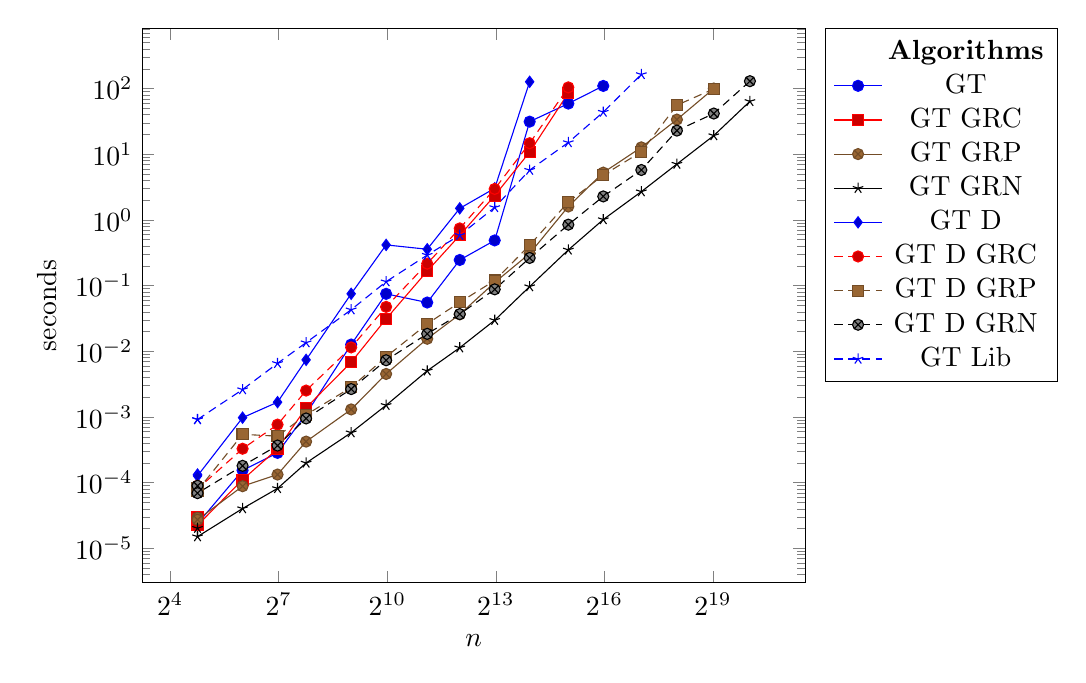
\begin{tikzpicture}
\begin{axis}[
    xlabel=$n$,ylabel=seconds,
    xmode=log,ymode=log,
    log basis x={2},
    legend style=
    {
        legend pos=outer north east
    },
    width=10cm
]
\addlegendimage{legend image code/.code=}
\legend{\textbf{Algorithms}, GT, GT GRC, GT GRP, GT GRN, GT D, GT D GRC, GT D GRP, GT D GRN, GT Lib}
\addplot table[x=n,y=value] {%GT
n value
27	2.54E-05
27	2.37646E-05
64	0.000153914
125	0.000284286
216	0.00111416
512	0.0126945
1000	0.075073033
2197	0.055363333
4096	0.245961333
8000	0.488409
15625	31.41703333
32768	59.17186667
64000	109.8606667
};
\addplot table[x=n,y=value] {%GT GRC
n value
27	3.03E-05
27	2.2432E-05
64	0.00011116
125	0.000326596
216	0.001382787
512	0.00682398
1000	0.031213833
2197	0.16648
4096	0.583621333
8000	2.351263333
15625	10.812
32768	85.61236667
};
\addplot table[x=n,y=value] {%GT GRP
n value
27	2.93E-05
27	2.73182E-05
64	8.83953E-05
125	0.000133037
216	0.000422432
512	0.00130516
1000	0.004525817
2197	0.0155378
4096	0.036563667
8000	0.111814333
15625	0.307891
32768	1.603586667
64000	5.25922
132651	12.75386667
262144	33.78733333
531441	100.2623333
};
\addplot table[x=n,y=value] {%GT GRN
n value
27	2.03E-05
27	1.51027E-05
64	4.04221E-05
125	8.18436E-05
216	0.000199778
512	0.000577347
1000	0.001509167
2197	0.005050763
4096	0.0113486
8000	0.0297681
15625	0.096823533
32768	0.350279
64000	1.014996667
132651	2.6983
262144	7.101253333
531441	19.29156667
1061208	64.0214
};
\addplot table[x=n,y=value] {%GT D
n value
27	1.33E-04
27	0.000127152
64	0.000977459
125	0.00168207
216	0.007420783
512	0.0751745
1000	0.417246
2197	0.358329333
4096	1.503013333
8000	3.035766667
15625	127.1716667
};
\addplot table[x=n,y=value] {%GT D GRC
n value
27	8.95E-05
27	8.04E-05
64	0.000328818
125	0.000766354
216	0.002527713
512	0.0114739
1000	0.0475249
2197	0.216508333
4096	0.744132
8000	2.9685
15625	14.74123333
32768	104.462
};
\addplot table[x=n,y=value] {%GT D GRP
n value
27	8.15E-05
27	7.59579E-05
64	0.000544588
125	0.000511051
216	0.001081957
512	0.002827437
1000	0.008248543
2197	0.026213167
4096	0.055797467
8000	0.119685667
15625	0.412618667
32768	1.87621
64000	4.814616667
132651	10.91256667
262144	55.88503333
531441	99.03183333
};
\addplot table[x=n,y=value] {%GT D GRN
n value
27	8.98E-05
27	0.000069295
64	0.000180789
125	0.000367908
216	0.000950806
512	0.00266219
1000	0.00731351
2197	0.018466767
4096	0.036885933
8000	0.0878232
15625	0.264105667
32768	0.848473667
64000	2.283013333
132651	5.76648
262144	22.9456
531441	41.73593333
1061208	129.805
};
\addplot table[x=n,y=value] {%GT Lib
n value
27	0.000922159
27	0.000915052
64	0.002620227
125	0.006562393
216	0.013568533
512	0.043020667
1000	0.114954
2197	0.291912667
4096	0.586437667
8000	1.553093333
15625	5.743833333
32768	15.12613333
64000	43.95683333
132651	164.3336667
};
\end{axis}
\end{tikzpicture}
\caption{Goldberg and Tarjan results from the GenRmf square graphs}
\label{fig:GenRmf square_GT_Results}
\end{figure}

An exception to the rule can be seen in Figure~\ref{fig:AK_GT_Results} which depicts GT results for AK graphs. 
Here, the dynamic tree version of the algorithms are slower, but coupled with the GRN heuristic, it is the fastest algorithm.
The big jump in the running time of the GT D GRN algorithm is due to an overflow error in the code. 
We expect the GT D GRN algorithm to behave like the KR LM D GRN algorithm in Figure~\ref{fig:AK_KR_Results} if the error is corrected.
We find that this speed-up is especially interesting, since adding dynamic trees or heuristics on their own makes the algorithm slower, but doing both gives a big speed-up.


\begin{figure}[h]
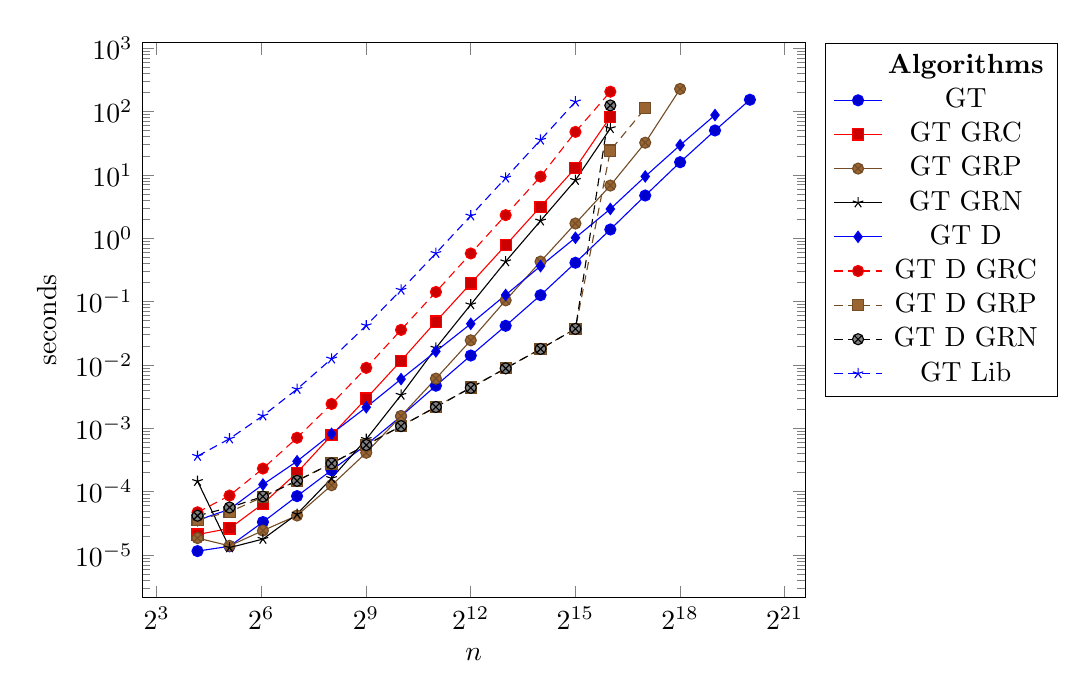
\begin{tikzpicture}
\begin{axis}[
    xlabel=$n$,ylabel=seconds,
    xmode=log,ymode=log,
    log basis x={2},
    legend style=
    {
        legend pos=outer north east
    },
    width=10cm
]
\addlegendimage{legend image code/.code=}
\legend{\textbf{Algorithms}, GT, GT GRC, GT GRP, GT GRN, GT D, GT D GRC, GT D GRP, GT D GRN, GT Lib}
\addplot table[x=n,y=value] {%GT
n value
18	1.15491E-05
34	1.37701E-05
66	3.32038E-05
130	8.51749E-05
258	0.000218989
514	0.000547029
1026	0.001555913
2050	0.004708267
4098	0.014102167
8194	0.041543667
16386	0.126403
32770	0.410714667
65538	1.375183333
131074	4.7243
262146	15.85233333
524290	50.24406667
1048578	153.437
};
\addplot table[x=n,y=value] {%GT GRC
n value
18	2.10994E-05
34	2.63187E-05
66	6.45197E-05
130	0.000200222
258	0.000779344
514	0.002955247
1026	0.011688167
2050	0.0483993
4098	0.193606
8194	0.774928333
16386	3.153233333
32770	12.85786667
65538	82.32676667
};
\addplot table[x=n,y=value] {%GT GRP
n value
18	1.85453E-05
34	1.39922E-05
66	2.43198E-05
130	4.20877E-05
258	0.000126596
514	0.000411993
1026	0.001565127
2050	0.006093057
4098	0.0244856
8194	0.104717
16386	0.428277667
32770	1.70907
65538	6.788133333
131074	32.18266667
262146	227.165
};
\addplot table[x=n,y=value] {%GT GRN
n value
18	0.000146252
34	1.31039E-05
66	0.000017879
130	4.43088E-05
258	0.00016291
514	0.000673739
1026	0.003355143
2050	0.018532733
4098	0.089804633
8194	0.429052667
16386	1.885126667
32770	8.247653333
65538	54.24016667
};
\addplot table[x=n,y=value] {%GT D
n value
18	3.54249E-05
34	5.28596E-05
66	0.000129928
130	0.00030261
258	0.000819102
514	0.002152143
1026	0.005989243
2050	0.016409467
4098	0.044628533
8194	0.127470333
16386	0.363211
32770	1.019396667
65538	2.897966667
131074	9.462753333
262146	29.41903333
524290	88.0256
};
\addplot table[x=n,y=value] {%GT D GRC
n value
18	4.73071E-05
34	8.68408E-05
66	0.000231983
130	0.000709607
258	0.002425103
514	0.009009903
1026	0.0358142
2050	0.142085333
4098	0.575261667
8194	2.315736667
16386	9.388776667
32770	47.68883333
65538	205.5886667
};
\addplot table[x=n,y=value] {%GT D GRP
n value
18	3.60912E-05
34	4.79734E-05
66	8.2621E-05
130	0.000149362
258	0.000279179
514	0.000546364
1026	0.00109295
2050	0.002178017
4098	0.00441367
8194	0.008896857
16386	0.017891767
32770	0.0374025
65538	24.21606667
131074	112.5863333
};
\addplot table[x=n,y=value] {%GT D GRN
n value
18	4.17547E-05
34	5.64132E-05
66	8.40646E-05
130	0.000148473
258	0.000279623
514	0.000545365
1026	0.001084287
2050	0.002170243
4098	0.00436003
8194	0.008836443
16386	0.0179194
32770	0.037174767
65538	124.819
};
\addplot table[x=n,y=value] {%GT Lib
n value
18	0.000364577
34	0.000685067
66	0.001577687
130	0.00415938
258	0.012518467
514	0.0419147
1026	0.152552
2050	0.579812333
4098	2.263826667
8194	8.971396667
16386	35.5501
32770	142.772
};
\end{axis}
\end{tikzpicture}
\caption{Goldberg and Tarjan results from the AK graphs}
\label{fig:AK_GT_Results}
\end{figure}

It is worth noting that we see a similar result for the KR algorithms on the AK graphs in Figure~\ref{fig:AK_KR_Results}. 
Here KR LM D GRN is significantly faster than all others. 
The reason the KR LM D GRP algorithm is slow is explained in Section~\ref{GRP Section}.

We did expect dynamic trees to perform well on the AK graphs, since they feature a very long path that has to be pushed on often. With dynamic trees, this can be done in logarithmic time instead of linear time.
In the other part of the graph however, without global relabelling, it will often push on very short paths which would be more efficient to just do directly. 
With global relabelling, we avoid pushing excess back and forth on these small paths. 
In fact, it creates a longer and longer path that is repeatability pushed on as the algorithm progresses. That is why the algorithm is so fast with heuristics and dynamic trees, but slow with just one of them.
The reason why GT D GRC is performing bad is due to the heuristic trigger, and will be explained in Section~\ref{Global Relabelling Section}.

Our conclusion with regard to dynamic tress is that algorithms only benefit from dynamic trees if the tree pushes mainly push on the same paths repeatability, and the paths are very long.
This generally does not occur, and we only found it in the AK graphs, which are very artificially constructed. On our more randomized graphs like GenRmf and Wash, we saw no improvements by using dynamic trees.

\subsection{Global Relabelling}
\label{Global Relabelling Section}

All of our heuristics perform the same basic global relabelling, but the triggers that determine when to run the global relabelling are different.
Regardless of the trigger, we always run a global relabelling at the start of the algorithm.



\begin{figure}[h]
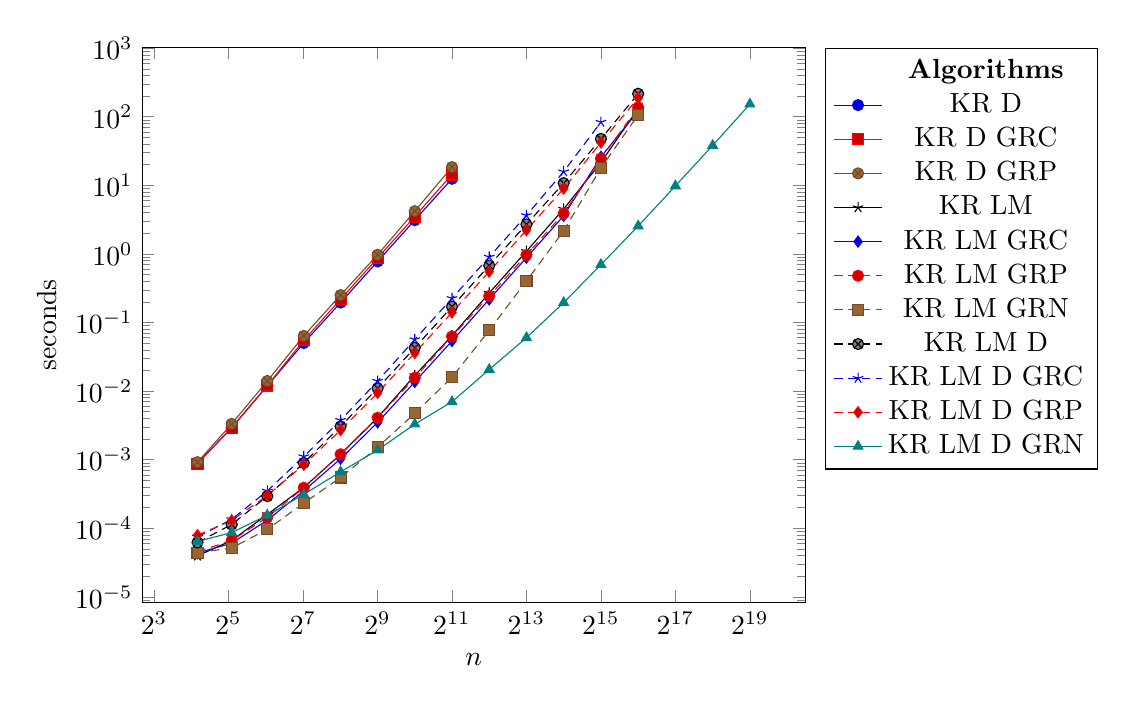
\begin{tikzpicture}
\begin{axis}[
    xlabel=$n$,ylabel=seconds,
    xmode=log,ymode=log,
    log basis x={2},
    legend style=
    {
        legend pos=outer north east
    },
    width=10cm
]
\addlegendimage{legend image code/.code=}
\legend{\textbf{Algorithms}, KR D, KR D GRC, KR D GRP, KR LM, KR LM GRC, KR LM GRP, KR LM GRN, KR LM D, KR LM D GRC, KR LM D GRP, KR LM D GRN}
\addplot table[x=n,y=value] {%KR
n value
18	0.000889175
34	0.002908057
66	0.011943033
130	0.050249867
258	0.195147333
514	0.777756
1026	3.107726667
2050	12.4823
};
\addplot table[x=n,y=value] {%KR GRC
n value
18	0.000875735
34	0.002938147
66	0.0120653
130	0.054935867
258	0.218274
514	0.872710333
1026	3.5095
2050	14.403
};
\addplot table[x=n,y=value] {%KR GRP
n value
18	0.000919492
34	0.00332838
66	0.014040333
130	0.0638248
258	0.251151333
514	0.971965333
1026	4.19931
2050	18.4658
};
\addplot table[x=n,y=value] {%KR LM
n value
18	3.95337E-05
34	6.66298E-05
66	0.000158912
130	0.000393449
258	0.00119856
514	0.00412505
1026	0.016918733
2050	0.064206667
4098	0.268975333
8194	1.09322
16386	4.51368
32770	21.53186667
65538	131.6553333
};
\addplot table[x=n,y=value] {%KR LM GRC
n value
18	4.34204E-05
34	6.07442E-05
66	0.000131261
130	0.000351139
258	0.001029877
514	0.00350173
1026	0.013609367
2050	0.0537659
4098	0.217405
8194	0.881691
16386	3.602213333
32770	26.04033333
65538	120.6886667
};
\addplot table[x=n,y=value] {%KR LM GRP
n value
18	4.57524E-05
34	6.62967E-05
66	0.000144697
130	0.000389451
258	0.00119834
514	0.00407752
1026	0.015643533
2050	0.062576267
4098	0.243189667
8194	0.966999333
16386	3.8901
32770	24.61043333
65538	136.8136667
};
\addplot table[x=n,y=value] {%KR LM GRN
n value
18	4.38646E-05
34	5.16381E-05
66	9.65021E-05
130	0.000232649
258	0.000549696
514	0.00151394
1026	0.00474304
2050	0.0158961
4098	0.0767171
8194	0.402905667
16386	2.16554
32770	17.93576667
65538	106.1156667
};
\addplot table[x=n,y=value] {%KR LM D
n value
18	6.21878E-05
34	0.000113493
66	0.000293837
130	0.000895949
258	0.003054753
514	0.010999333
1026	0.0427871
2050	0.170356
4098	0.676120333
8194	2.693893333
16386	10.74853333
32770	47.54073333
65538	216.514
};
\addplot table[x=n,y=value] {%KR LM D GRC
n value
18	7.48474E-05
34	0.000134814
66	0.000350584
130	0.00111305
258	0.003765693
514	0.014000933
1026	0.0564863
2050	0.225324667
4098	0.904017333
8194	3.646476667
16386	15.8397
32770	83.65686667
};
\addplot table[x=n,y=value] {%KR LM D GRP
n value
18	7.94004E-05
34	0.000130039
66	0.000300056
130	0.000844977
258	0.002696287
514	0.009420677
1026	0.035984667
2050	0.140029
4098	0.551803333
8194	2.21699
16386	8.955463333
32770	42.12056667
65538	186.7876667
};
\addplot[mark=triangle*, teal] table[x=n,y=value] {%KR LM D GRN
n value
18	6.41867E-05
34	8.66187E-05
66	0.00015447
130	0.000312605
258	0.000664521
514	0.001379017
1026	0.003295733
2050	0.006980693
4098	0.020601467
8194	0.0600087
16386	0.194730333
32770	0.69788
65538	2.548136667
131074	9.800743333
262146	38.14566667
524290	152.5736667
};
\end{axis}
\end{tikzpicture}
\caption{King and Rao results from the AK graphs}
\label{fig:AK_KR_Results}
\end{figure}


All of our heuristics perform worse than no heuristics on the CD graphs. This is because it is never needed to send flow back to the source in the CD graph.
None of the global relabels runs relabel any nodes significantly up. 
The AK graphs also do not require any excess to be routed back, but here GT D GRP and GT D GRN are faster than all other GT algorithms.
Likewise, KR LM D GRN is faster than other KR algorithms. This can be seen from Figure~\ref{fig:AK_GT_Results} and Figure~\ref{fig:AK_KR_Results}.
The left side of the AK graphs as depicted in Figure~\ref{akExample} from Section~\ref{AKGraphSection} still cause flow to be pushed back and forth if no global relabelling is done however.


\subsubsection{GRC}

The first heuristic we implemented was the GRC heuristic. It does a global relabelling whenever a node is relabelled more than one label up.
It performs very well on the CRH graphs, but not very well on AK graphs. On GenRmf and Wash graphs, they are more stable than not using heuristics, and generally slightly faster.
The reason we implemented the heuristic was that the running time of the algorithms was very unstable in the GenRmf and Wash graphs, so we did expect the heuristic to be more stable and faster on those graphs.
Examples of the instability in the algorithms without global relabelling can be seen in Figure~\ref{fig:GenRmf long_GT_Results} and Figure~\ref{fig:GenRmf long_KR_Results}.

CRH graphs are the best case graphs for this particular trigger. As soon as the last edge to $t$ is saturated, that node will have to be relabelled twice since all other nodes have a higher label than it does.
That triggers the global relabel, and the excess is then sent to $s$. If you consider the AK graphs however, the square pattern on the left side as depicted in Figure~\ref{akExample} from Section~\ref{AKGraphSection} causes the heuristic to trigger very often.
After the first global relabel, all nodes is labelled according to their distance to $t$. Excess is then pushed from the first node in the lower part of the left side to the top part of the left side and on to $t$.
For the algorithm to continue here, excess must be pushed to the next node in the lower part of the left side. This requires that the first node in the lower part is relabelled twice, even though nothing has been pushed in a cycle.
The global relabel is not going to change any labels on the left side, so it is just wasted effort.
This happens again and again each time flow is pushed further along the lower part of the left side.
The performance on CRH and AK graphs can be seen in Appendix~\ref{ChartAppendix}.

This triggering of the heuristic when there are no cycles is why we decided to implement the GRP trigger.

\subsubsection{GRP}
\label{GRP Section}

The GRP trigger triggers when flow has not been sent to the target since the last pass, if flow has been sent to the target since the last global relabelling.
This gave a major speed-up for the GT algorithms on GenRmf and Wash graphs. This can for instance be seen in Figure~\ref{fig:GenRmf square_GT_Results}. 
As discussed in Section~\ref{Dynamic Trees Section}, GT D GRP gained major speed-ups on the AK graphs as well.

As can be seen from Figure~\ref{fig:GenRmf long_KR_Results}, we did not see any major speed-ups for the KR algorithms when using the GRP heuristic instead of the GRC heuristic. 
Due to the way edges are added in the KR algorithm, there are not many active nodes at a time in the KR algorithm.
When an edge $(u, v)$ is added, it might cause the visible excess of $u$ become positive and activate the node.
This causes the excess to be pushed around the graph, which might activate other nodes.
The number of nodes that are active at the same time remain low though, which means the global relabelling check is called very often.
A result of this is that the KR algorithms with the GRP heuristic perform a global relabel every time the excess of $t$ changes.

To get a more consistent speed-up, we decided to base the trigger off the number of nodes processed instead of passes, which lead to the GRN heuristic.

\subsubsection{GRN}

Instead of checking the excess of $t$ after each pass, the GRN heuristic does it after $f(G)$ nodes have been processed.
This improved upon the running times for the GT and KR algorithms on the AK, GenRmf and Wash graphs.
For examples of this, see Figures 
\ref{fig:GenRmf long_GT_Results}, 
\ref{fig:GenRmf long_KR_Results}, 
\ref{fig:GenRmf square_GT_Results}, 
\ref{fig:AK_GT_Results}, 
\ref{fig:AK_KR_Results}, 
or Appendix~\ref{ChartAppendix}.

\subsection{Library Implementations}

We tested a set of max flow algorithms from the C++ Boost Library \cite{BoostLibraries}.
It has implementations for the Edmonds and Karp algorithm, the Goldberg and Tarjan algorithm, and an algorithm by Boykov and Kolmogorov.
The Boykov and Kolmogorov algorithm is an algorithm that is designed to be efficient on a special type of max flow graphs that arise from computer vision.

We tested the algorithms on all of our graphs, and found that the library algorithms are relatively slow.
The library implementation of the Edmonds and Karp algorithm is almost 100 times slower than our implementation, even though we have not done any significant optimizations to it.
The implementation of the Goldberg and Tarjan algorithm is also slow compared to our implementations. 
If you look at Figure~\ref{fig:GenRmf square_GT_Results}, you can see that GT Lib is about the same time as our implementations without heuristics or with the GRC heuristic.
It is slower for small graphs, and faster for larger graphs. The slope is about the same as our algorithms with the GRN heuristic, but it is again about 100 times slower.
The slope and lack of jumps tell us that they do use some form of heuristics to detect when the min cut is saturated.
We have profiled it to ensure that it is not something in our code that is causing the slowdown, but all the work is done in functions inside the boost library.

As for the BK Lib algorithm, if we compare it to GT Lib, then BK Lib is faster on small graphs, and GT tends to win as the graphs become bigger.
It is still far behind our best algorithms on all graphs.


\begin{figure}[h]
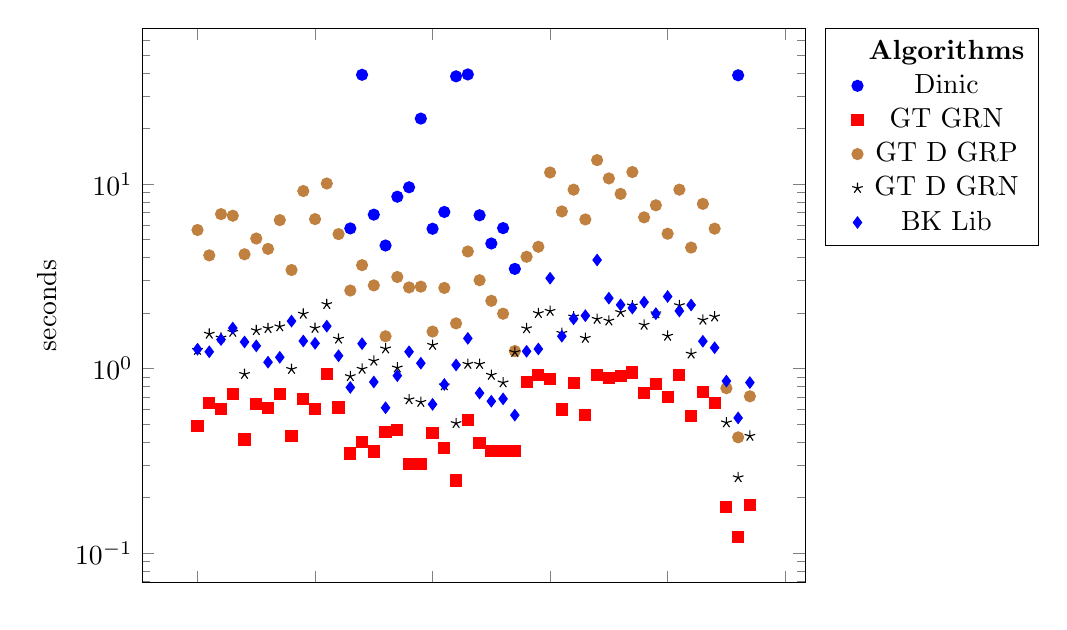
\begin{tikzpicture}
\begin{axis}[
    ylabel=seconds,ymode=log,
	symbolic x coords={BVZ-sawtooth04,BVZ-sawtooth06,BVZ-sawtooth07,BVZ-sawtooth08,BVZ-sawtooth09,BVZ-sawtooth10,BVZ-sawtooth11,BVZ-sawtooth12,BVZ-sawtooth13,BVZ-sawtooth14,BVZ-sawtooth15,BVZ-sawtooth16,BVZ-sawtooth18,BVZ-tsukuba00,BVZ-tsukuba01,BVZ-tsukuba02,BVZ-tsukuba03,BVZ-tsukuba04,BVZ-tsukuba05,BVZ-tsukuba6,BVZ-tsukuba7,BVZ-tsukuba8,BVZ-tsukuba9,BVZ-tsukuba10,BVZ-tsukuba11,BVZ-tsukuba12,BVZ-tsukuba14,BVZ-tsukuba15,BVZ-venus01,BVZ-venus02,BVZ-venus03,BVZ-venus04,BVZ-venus05,BVZ-venus06,BVZ-venus07,BVZ-venus08,BVZ-venus09,BVZ-venus10,BVZ-venus11,BVZ-venus12,BVZ-venus13,BVZ-venus14,BVZ-venus15,BVZ-venus16,BVZ-venus17,KZ2-sawtooth17,KZ2-tsukuba13,KZ2-venus19},
	xticklabels={,,},
    legend style=
    {
        legend pos=outer north east
    },
    width=10cm
]
\addlegendimage{legend image code/.code=}
\legend{\textbf{Algorithms}, Dinic, GT GRN, GT D GRP, GT D GRN, BK Lib}
\addplot[only marks, blue, mark=*] table[x=n,y=value] {%Dinic
n value
BVZ-tsukuba00	5.750836667
BVZ-tsukuba01	39.14823333
BVZ-tsukuba02	6.83006
BVZ-tsukuba03	4.645143333
BVZ-tsukuba04	8.541403333
BVZ-tsukuba05	9.609163333
BVZ-tsukuba10	39.3178
BVZ-tsukuba11	6.7765
BVZ-tsukuba12	4.763366667
BVZ-tsukuba14	5.771553333
BVZ-tsukuba15	3.468896667
BVZ-tsukuba6	22.6535
BVZ-tsukuba7	5.724696667
BVZ-tsukuba8	7.061796667
BVZ-tsukuba9	38.3952
KZ2-tsukuba13	38.90546667
};
\addplot[only marks, red, mark=square*] table[x=n,y=value] {%GT GRN
n value
BVZ-sawtooth04	0.489767333
BVZ-sawtooth06	0.650722667
BVZ-sawtooth07	0.602036667
BVZ-sawtooth08	0.728916
BVZ-sawtooth09	0.412417333
BVZ-sawtooth10	0.642597
BVZ-sawtooth11	0.610116
BVZ-sawtooth12	0.731337
BVZ-sawtooth13	0.429253333
BVZ-sawtooth14	0.683659333
BVZ-sawtooth15	0.604143
BVZ-sawtooth16	0.933819
BVZ-sawtooth18	0.614827667
BVZ-tsukuba00	0.346019
BVZ-tsukuba01	0.39826
BVZ-tsukuba02	0.355036667
BVZ-tsukuba03	0.452382667
BVZ-tsukuba04	0.462989667
BVZ-tsukuba05	0.302774
BVZ-tsukuba10	0.523340333
BVZ-tsukuba11	0.394437667
BVZ-tsukuba12	0.357265333
BVZ-tsukuba14	0.356760667
BVZ-tsukuba15	0.358245
BVZ-tsukuba6	0.30229
BVZ-tsukuba7	0.447588333
BVZ-tsukuba8	0.371264
BVZ-tsukuba9	0.247241333
BVZ-venus01	0.844272667
BVZ-venus02	0.918598
BVZ-venus03	0.873629667
BVZ-venus04	0.599272
BVZ-venus05	0.836556333
BVZ-venus06	0.559744667
BVZ-venus07	0.920171667
BVZ-venus08	0.885694
BVZ-venus09	0.912648
BVZ-venus10	0.951088333
BVZ-venus11	0.740437333
BVZ-venus12	0.821746
BVZ-venus13	0.702746333
BVZ-venus14	0.926211
BVZ-venus15	0.550986667
BVZ-venus16	0.742330333
BVZ-venus17	0.649391333
KZ2-sawtooth17	0.177902
KZ2-tsukuba13	0.12262
KZ2-venus19	0.181196667
};
\addplot[only marks, brown, mark=oplus*] table[x=n,y=value] {%GT D GRP
n value
BVZ-sawtooth04	5.637843333
BVZ-sawtooth06	4.106903333
BVZ-sawtooth07	6.87372
BVZ-sawtooth08	6.738953333
BVZ-sawtooth09	4.163056667
BVZ-sawtooth10	5.067443333
BVZ-sawtooth11	4.45305
BVZ-sawtooth12	6.378663333
BVZ-sawtooth13	3.42055
BVZ-sawtooth14	9.17015
BVZ-sawtooth15	6.45878
BVZ-sawtooth16	10.07306667
BVZ-sawtooth18	5.355506667
BVZ-tsukuba00	2.647463333
BVZ-tsukuba01	3.635553333
BVZ-tsukuba02	2.823506667
BVZ-tsukuba03	1.495733333
BVZ-tsukuba04	3.1349
BVZ-tsukuba05	2.75291
BVZ-tsukuba10	4.310993333
BVZ-tsukuba11	3.01142
BVZ-tsukuba12	2.328253333
BVZ-tsukuba14	1.98249
BVZ-tsukuba15	1.243746667
BVZ-tsukuba6	2.779606667
BVZ-tsukuba7	1.58586
BVZ-tsukuba8	2.73537
BVZ-tsukuba9	1.757243333
BVZ-venus01	4.034523333
BVZ-venus02	4.57276
BVZ-venus03	11.55953333
BVZ-venus04	7.10882
BVZ-venus05	9.328716667
BVZ-venus06	6.432303333
BVZ-venus07	13.49126667
BVZ-venus08	10.73153333
BVZ-venus09	8.848846667
BVZ-venus10	11.6229
BVZ-venus11	6.6005
BVZ-venus12	7.675843333
BVZ-venus13	5.381833333
BVZ-venus14	9.32988
BVZ-venus15	4.527093333
BVZ-venus16	7.814476667
BVZ-venus17	5.7328
KZ2-sawtooth17	0.782533333
KZ2-tsukuba13	0.42346
KZ2-venus19	0.706977667
};
\addplot[only marks, black, mark=star] table[x=n,y=value] {%GT D GRN
n value
BVZ-sawtooth04	1.257363333
BVZ-sawtooth06	1.5395
BVZ-sawtooth07	1.467783333
BVZ-sawtooth08	1.575723333
BVZ-sawtooth09	0.931440667
BVZ-sawtooth10	1.60887
BVZ-sawtooth11	1.65183
BVZ-sawtooth12	1.687383333
BVZ-sawtooth13	0.991900333
BVZ-sawtooth14	1.97617
BVZ-sawtooth15	1.65473
BVZ-sawtooth16	2.2296
BVZ-sawtooth18	1.4468
BVZ-tsukuba00	0.906884333
BVZ-tsukuba01	0.993645333
BVZ-tsukuba02	1.099296667
BVZ-tsukuba03	1.280756667
BVZ-tsukuba04	1.009479333
BVZ-tsukuba05	0.679007
BVZ-tsukuba10	1.05689
BVZ-tsukuba11	1.0557
BVZ-tsukuba12	0.921605
BVZ-tsukuba14	0.837999333
BVZ-tsukuba15	1.225756667
BVZ-tsukuba6	0.657387333
BVZ-tsukuba7	1.33941
BVZ-tsukuba8	0.807863333
BVZ-tsukuba9	0.504580667
BVZ-venus01	1.648326667
BVZ-venus02	1.992683333
BVZ-venus03	2.047933333
BVZ-venus04	1.555906667
BVZ-venus05	1.909363333
BVZ-venus06	1.461823333
BVZ-venus07	1.853596667
BVZ-venus08	1.81487
BVZ-venus09	2.017216667
BVZ-venus10	2.190356667
BVZ-venus11	1.721903333
BVZ-venus12	1.98797
BVZ-venus13	1.501023333
BVZ-venus14	2.19958
BVZ-venus15	1.20103
BVZ-venus16	1.834053333
BVZ-venus17	1.909196667
KZ2-sawtooth17	0.508664
KZ2-tsukuba13	0.256661
KZ2-venus19	0.430539333
};
\addplot[only marks, blue, mark=diamond*] table[x=n,y=value] {%BK Lib
n value
BVZ-sawtooth04	1.272543333
BVZ-sawtooth06	1.23261
BVZ-sawtooth07	1.43546
BVZ-sawtooth08	1.65753
BVZ-sawtooth09	1.39307
BVZ-sawtooth10	1.32683
BVZ-sawtooth11	1.082433333
BVZ-sawtooth12	1.150216667
BVZ-sawtooth13	1.807283333
BVZ-sawtooth14	1.409916667
BVZ-sawtooth15	1.36928
BVZ-sawtooth16	1.69699
BVZ-sawtooth18	1.172643333
BVZ-tsukuba00	0.789907667
BVZ-tsukuba01	1.363463333
BVZ-tsukuba02	0.844900667
BVZ-tsukuba03	0.612848667
BVZ-tsukuba04	0.914284667
BVZ-tsukuba05	1.232753333
BVZ-tsukuba10	1.457013333
BVZ-tsukuba11	0.736029333
BVZ-tsukuba12	0.664695333
BVZ-tsukuba14	0.684720333
BVZ-tsukuba15	0.559057667
BVZ-tsukuba6	1.068726667
BVZ-tsukuba7	0.639465
BVZ-tsukuba8	0.819790667
BVZ-tsukuba9	1.045543333
BVZ-venus01	1.240246667
BVZ-venus02	1.27637
BVZ-venus03	3.08739
BVZ-venus04	1.497496667
BVZ-venus05	1.8612
BVZ-venus06	1.934973333
BVZ-venus07	3.87581
BVZ-venus08	2.406416667
BVZ-venus09	2.214203333
BVZ-venus10	2.129076667
BVZ-venus11	2.290323333
BVZ-venus12	1.983696667
BVZ-venus13	2.456886667
BVZ-venus14	2.050246667
BVZ-venus15	2.21068
BVZ-venus16	1.405656667
BVZ-venus17	1.296033333
KZ2-sawtooth17	0.855298667
KZ2-tsukuba13	0.539781667
KZ2-venus19	0.839086
};
\end{axis}
\end{tikzpicture}
\caption{Results from the Computer Vision graphs}
\label{fig:CV_Results}
\end{figure}

To get some graphs that BK Lib should work well on, we found some max flow graphs that are generated from computer vision problems \cite{CVGraphsSite}.
The graphs are rather big, so we have not been able to run all of our algorithms on them, but GT GRN, GT D GRP, GT D GRN and BK Lib all perform well enough for us to get data on them within reasonable time.
The data for the CV graphs can be seen in Figure~\ref{fig:CV_Results}.
When we ran the tests, we ran each algorithms on the graphs for 15 minutes. The order the graphs were tested was sorted by file size on disk, 
but in in Figure~\ref{fig:CV_Results} the points are alphabetically sorted.
From left to right, the chart contains data for BVZ-sawtooth number 4, 6-16 and 18, BVZ-tsukuba number 0-15, BVZ-venus number 1-17, and the graphs KZ2-sawtooth17, KZ2-tsukuba13 and KZ2-venus19.

As expected, the BK Lib algorithm performs quite well on these graphs.
It is not fast enough to beat GT GRN, but it is the second fastest algorithm we have tested.

\section{Future Works}
If we had more time, we would have liked to spend more time optimizing our algorithms.
We believe that there is still room for improvements in experimenting with some of the parameters in the algorithms.

Also, better algorithms for routing the blocking flow in Dinic might speed up this algorithm.
A problem with Dinic right now is that it might process the same part of the layer graph multiple times.
It might be possible to speed it up by saving information about the paths in the layer graph that has already been visited once.
One way of doing this could be using dynamic trees, but we have not seen a big improvement for the other algorithms when using dynamic trees.
That having been said, layer graphs does tend to be long paths with reusable edges, so we could see a good performance boost by adding dynamic trees.
Alternatively, we could use the push pull block algorithm that is used in Goldberg Rao to compute the blocking flow, which would also reduce the theoretical running time to $O\left(nm\log{\frac{n^2}{m}}\right)$.

As mentioned in Section~\ref{ImplementationSection}, we could probably gain some performance by using templates for custom data in nodes instead of a pointer to an object containing the custom data.
A graph node takes up 24 bytes, and an edge takes 32 bytes. With a cache line of 64 bytes, this means we load about two nodes with every cache miss.
The probability that we need the other node is low however as proximity in memory does not imply proximity in the graph.
Even if the first node has an edge to the other node, it probably has edges to other nodes as well.
In the table below we listed the sizes for some of the objects in our algorithms.
\begin{table}[h]
\centering
\begin{tabular}{|l|r|r|}
\hline
\multicolumn{1}{|l}{Object} &
\multicolumn{1}{|l}{Size} &
\multicolumn{1}{|l|}{Padding} \\\hline
Node&24 bytes & 4 bytes\\\hline
Edge&32 bytes & 4 bytes\\\hline
EK Node Tag & 16 bytes & 0 bytes\\\hline
Dinic Node Tag & 24 bytes & 0 bytes\\\hline
GT Node Tag & 24 bytes & 4 bytes\\\hline
GT D Node Tag & 32 bytes & 4 bytes\\\hline
KR LM Node Tag & 128 bytes & 4 bytes\\\hline
Dynamic Tree Node & 80 bytes & 0 bytes\\\hline
\end{tabular}
\end{table}\\
Variables are aligned to start on an address that is a multiple of their size. For instance, a 4 byte variable can start on address $4, 8, 12$ etc.
Variables are aligned by padding the previous variable. For instance, if we define a 32 bit variable followed by a 64 bit variable, 
the 32 bit variable will be padded to 64 bit so the 64 bit variable starts at a multiple of 8.
To allow putting structs next to each other in an array, the struct is also padded so that its size is a multiple of the size of the biggest primitive in it.
For instance, we use 64 bit pointers, which means that any struct that contains a pointer is padded so that its size in bytes is a multiple of 8.
Padding to align variables can generally be avoided by defining them in order of biggest to smallest.
The size column specifies the total size of the object, and the padding column specifies how much of that is padding. 
This means that if we were to merge two objects each of size 24 bytes with 4 bytes of padding, we would be able to merge those to an object of size 40 bytes with no padding.
Additionally, merging a tag with the node removes the need for the pointer in the node to the tag.

What is interesting about this table is that node tags from all algorithms except from KR can be merged with the graph node into an object that fits into one cache line.
In fact, merging GT results in an object that takes up 24 bytes from the node, 24 bytes from the GT tag, minus 8 bytes from padding, and minus 8 bytes for one less pointer in the node.
In total, 32 bytes. That means that two nodes would fit perfectly into one cache line. 
We went up to 64 bit pointers due to memory issues in KR, but with 32 bit pointers, a merged graph node and GT D node tag would take up 28 bytes.
This would also allow for GT D to place two merged nodes in one cache line.
Since 28 bytes is not a perfect half cache line though, $1/4$ of the nodes will be placed to span two cache lines.
It might be worth it to pad these nodes with an extra 4 bytes so that no nodes span two cache lines.

The KR tags take up a lot of memory because they need to contain the game in them, which means a lot of linked lists.
This means that we would not be able to read an entire node in one cache line, but we would still expect to see a performance increase.
The reason is that the CPU could load the information it needs directly instead of having to load a pointer and then load the information it needs.

As mentioned before, the downside of this optimization is that the graph needs to be cloned. 
For graphs such as CRE and CRH, that is probably not worth it due to the large number of edges that do not need to be used, but we would expect to see a speed up on our other graphs.

We have not had much time to optimize the Goldberg Rao algorithm, so more work on that could bring its running time down.

Finally, it would be interesting to implement Orlin and compare it to the other algorithms. 
We don't expect it will be faster though, since it adds a lot of complexity and memory use.

\section{Conclusion}

Although we did not get to implementing the Orlin algorithm \cite{Orlin13} as we had hoped, we did get some interesting results.
Our contribution to the algorithm by King and Rao is not only a theoretical result, but it also makes a big difference in practice.
The addition to the Goldberg Rao theory fixes an issue it has with one of its assumptions, and make the theory hold.

On the performance side of things, we can conclude that a naive implementation of the algorithm by Dinic is often better than a naive implementation of the other algorithms.
However, we found more room for optimizations and heuristics on the Push-Relabel algorithms such as the algorithms by Goldberg and Tarjan, and by King and Rao.
We did not find the added complexity of the King Rao algorithms in relation to the Goldberg Tarjan algorithms to be worth it however.
Likewise, the algorithms do for the most part not benefit from dynamic trees.
It appears as though the Goldberg Rao algorithm has too many different things going on for it to be really efficient, but there is room for optimizations in our implementation.

























































